\chapter{INSTALLATION}
\section{Prerequisite}
\tocless\subsection{Node.js}
\begin{enumerate}
	\item Download Node.js installer from \href{https://nodejs.org/en/download/}{its official download page}
	      \begin{center}
	      	\begin{figure}[H]
	      		\centering
	      		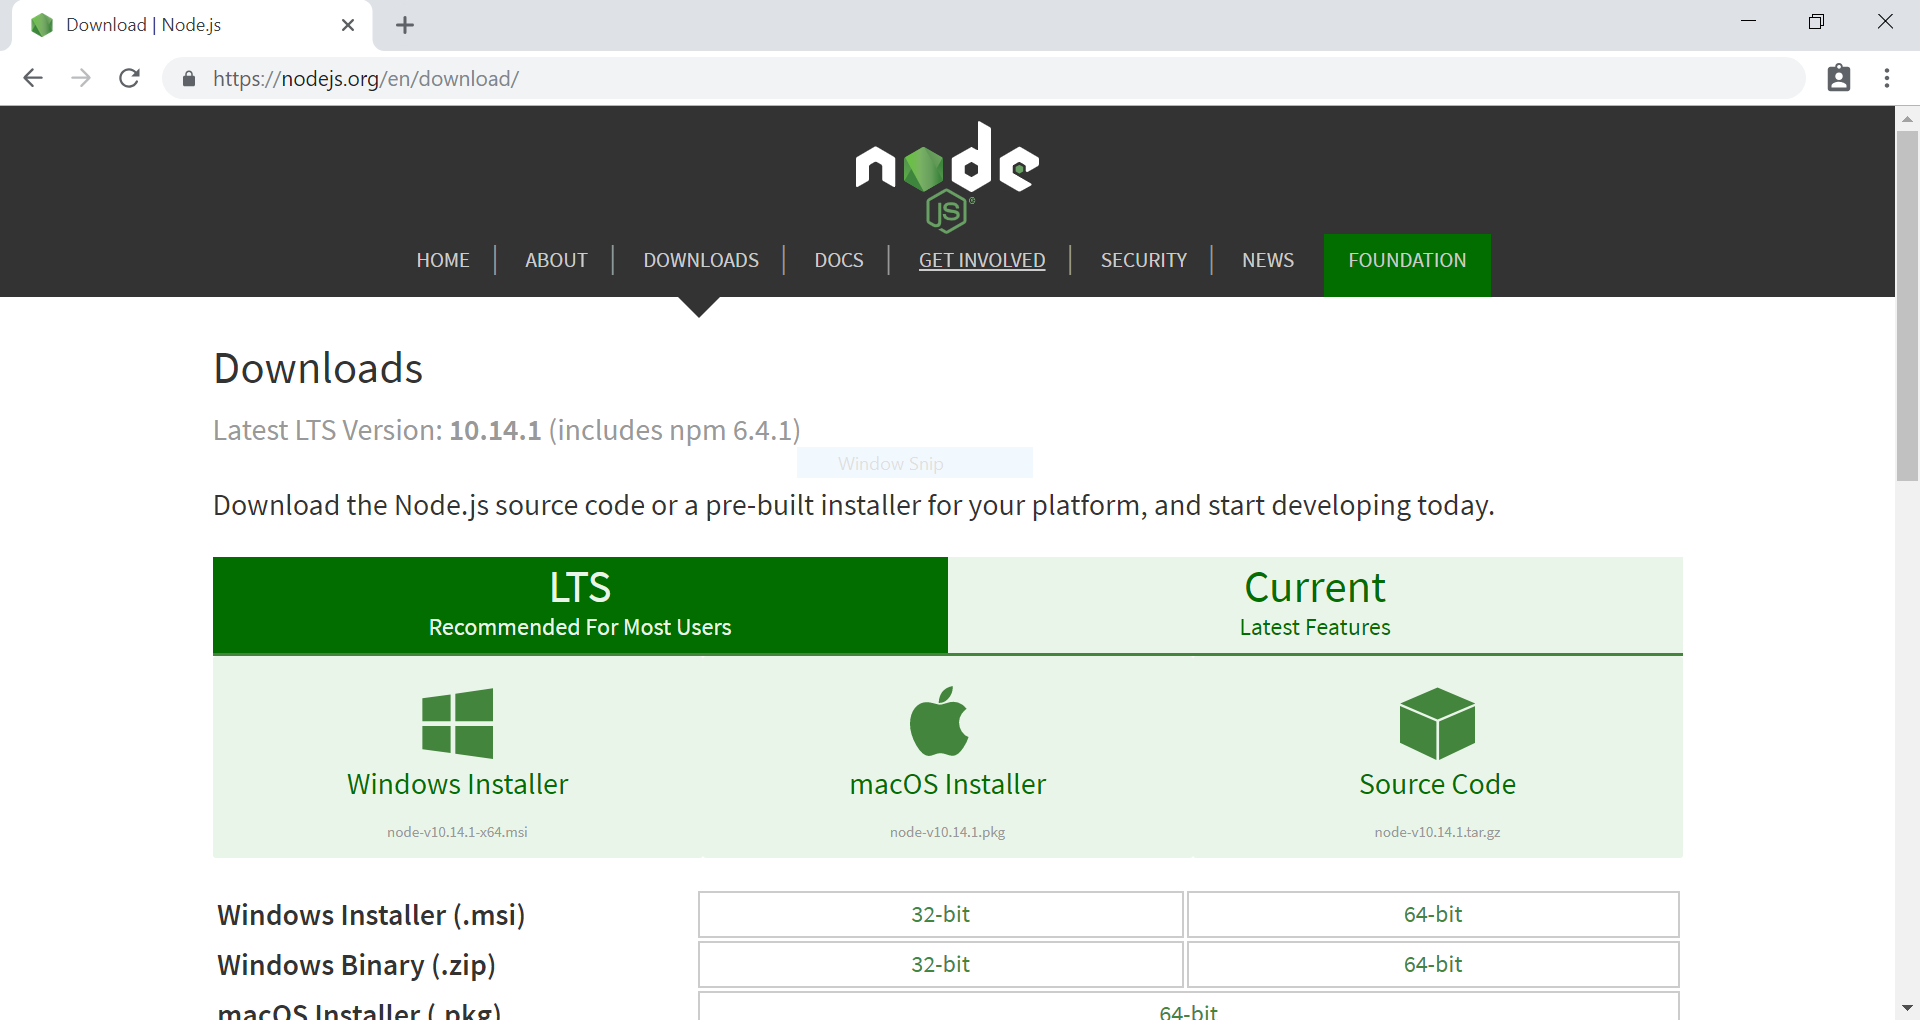
\includegraphics[width=0.6\columnwidth]{images/appendixA/Nodejs-download-page.PNG}
	      		\footcaption{Node.js official download page}
	      	\end{figure}
	      \end{center}
	      \footnotetext{Source: \url{https://nodejs.org/en/download/}} 
	\item Follow the instruction of setup wizard and install Node.js
	      \begin{center}
	      	\begin{figure}[H]
	      		\centering
	      		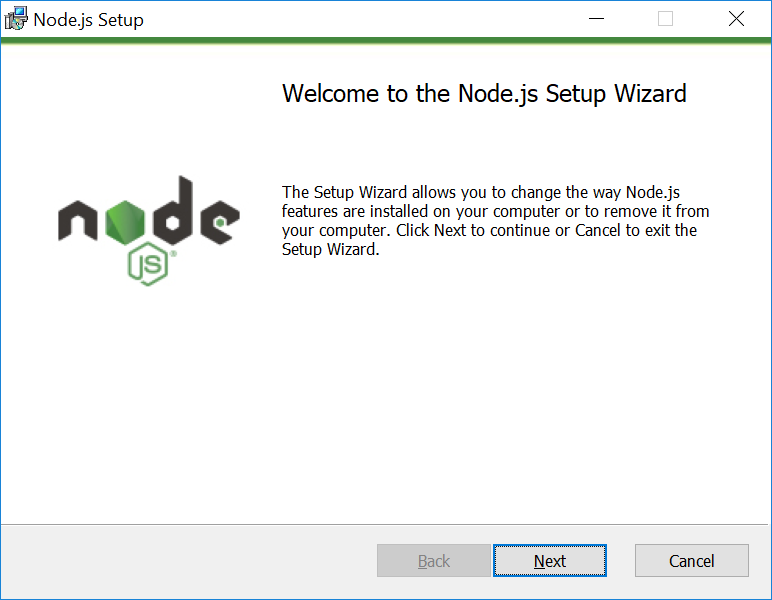
\includegraphics[width=0.6\columnwidth]{images/appendixA/Nodejs-setup.PNG}
	      		\footcaption{Node.js Setup Wizard}
	      	\end{figure}
	      \end{center}
	      \footnotetext{Source: Node.js Setup Wizard} 
	\item To verify installation, open \textit{Window Command Prompt} and enter following command: \verb+node -v+
	      \begin{center}
	      	\begin{figure}[H]
	      		\centering
	      		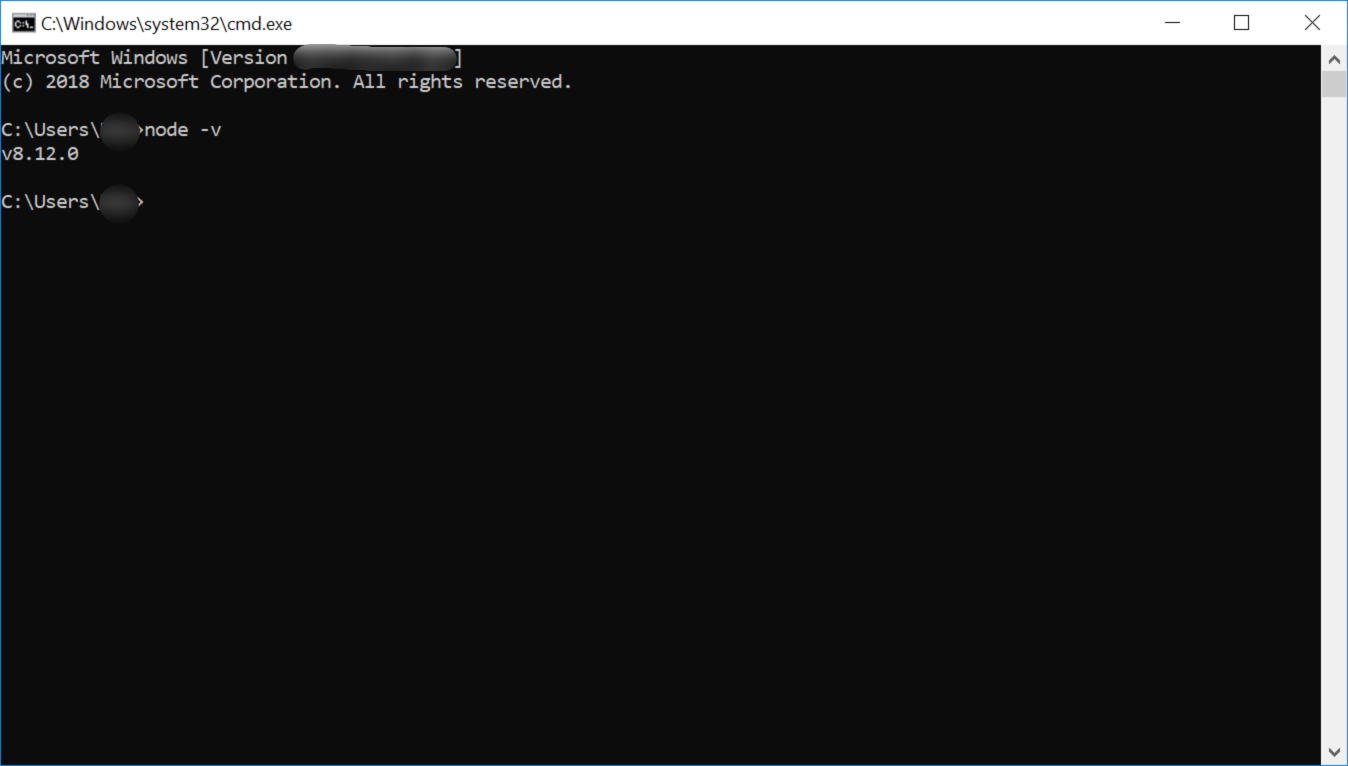
\includegraphics[width=0.6\columnwidth]{images/appendixA/Nodejs-verify-install.PNG}
	      		\footcaption{Node.js installation verification}
	      	\end{figure}
	      \end{center}
	      \footnotetext{Source: Window Command Prompt} 
\end{enumerate}
\tocless\subsection{Google Cloud Platform}
\begin{enumerate}
	\item Create an account and a new project on \textit{Google Cloud Platform} from \href{https://cloud.google.com/}{here}
	      \begin{center}
	      	\begin{figure}[H]
	      		\centering
	      		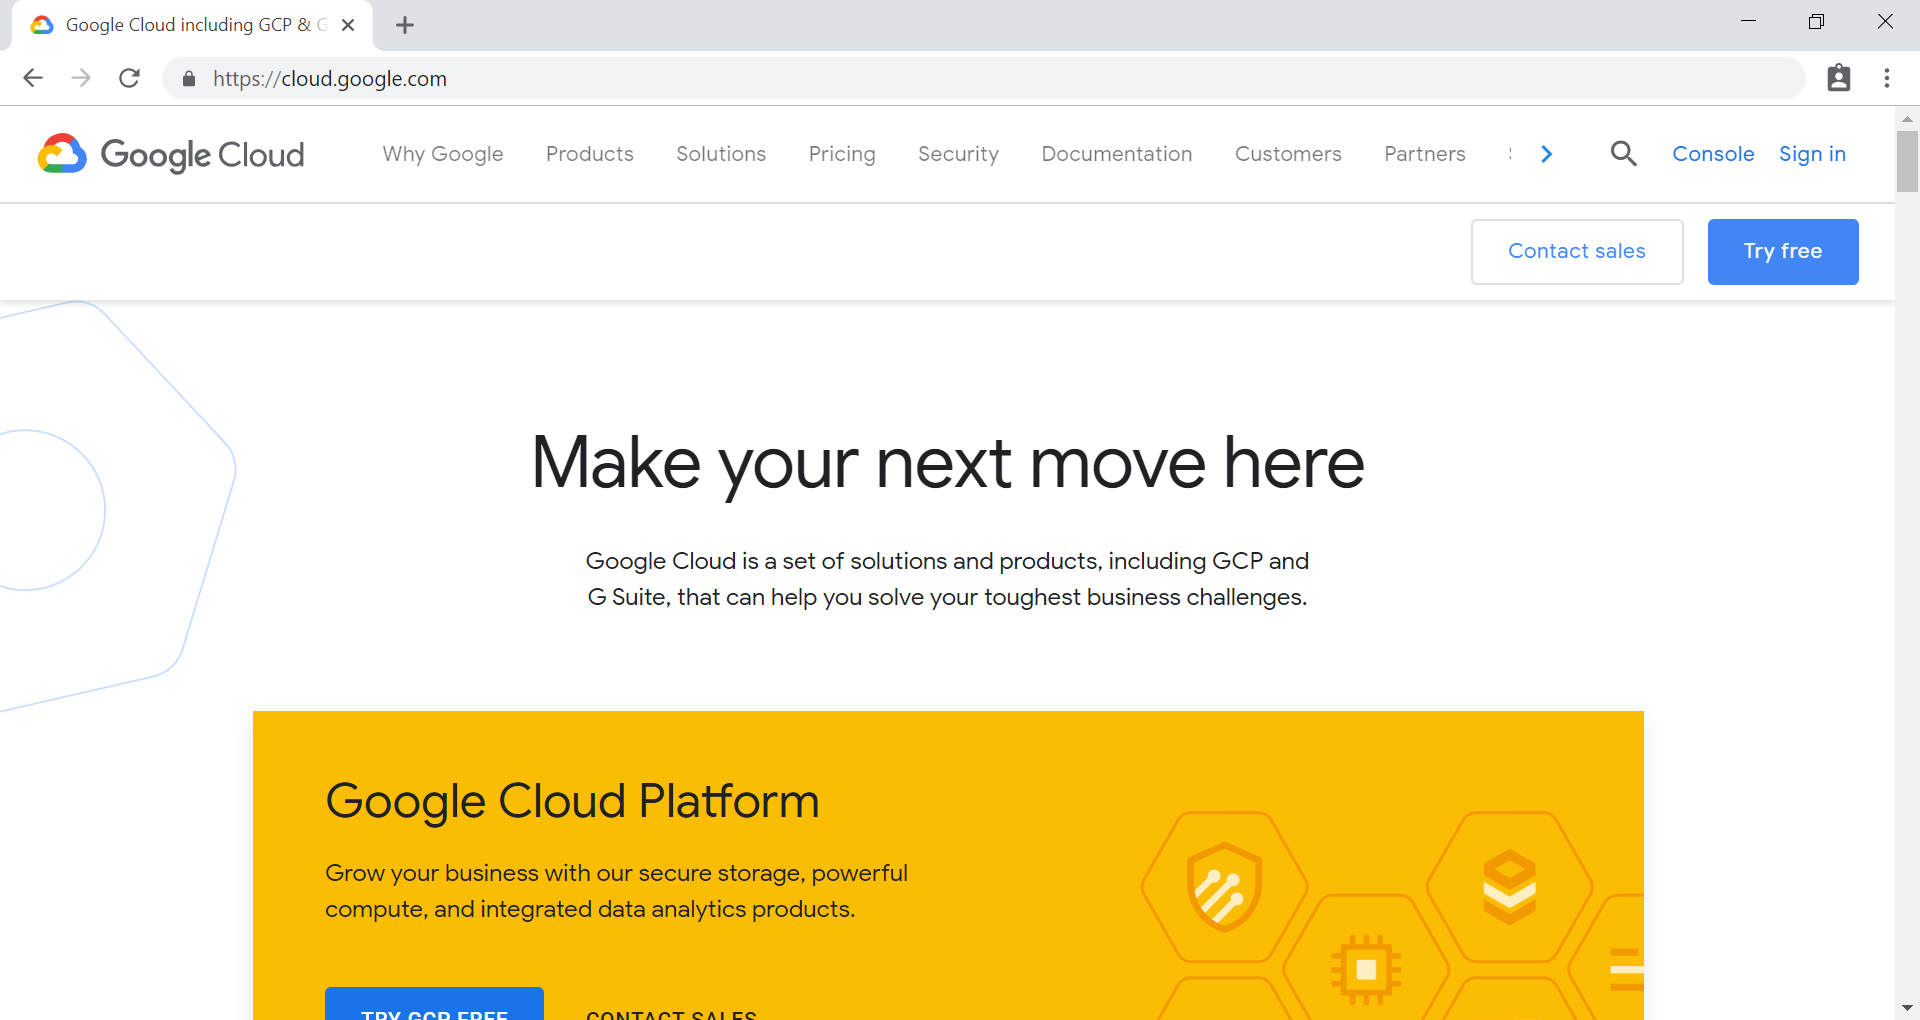
\includegraphics[width=0.6\columnwidth]{images/appendixA/GCP-homepage.PNG}
	      		\footcaption{Google Cloud Platform homepage}
	      	\end{figure}
	      \end{center}
	      \begin{center}
	      	\begin{figure}[H]
	      		\centering
	      		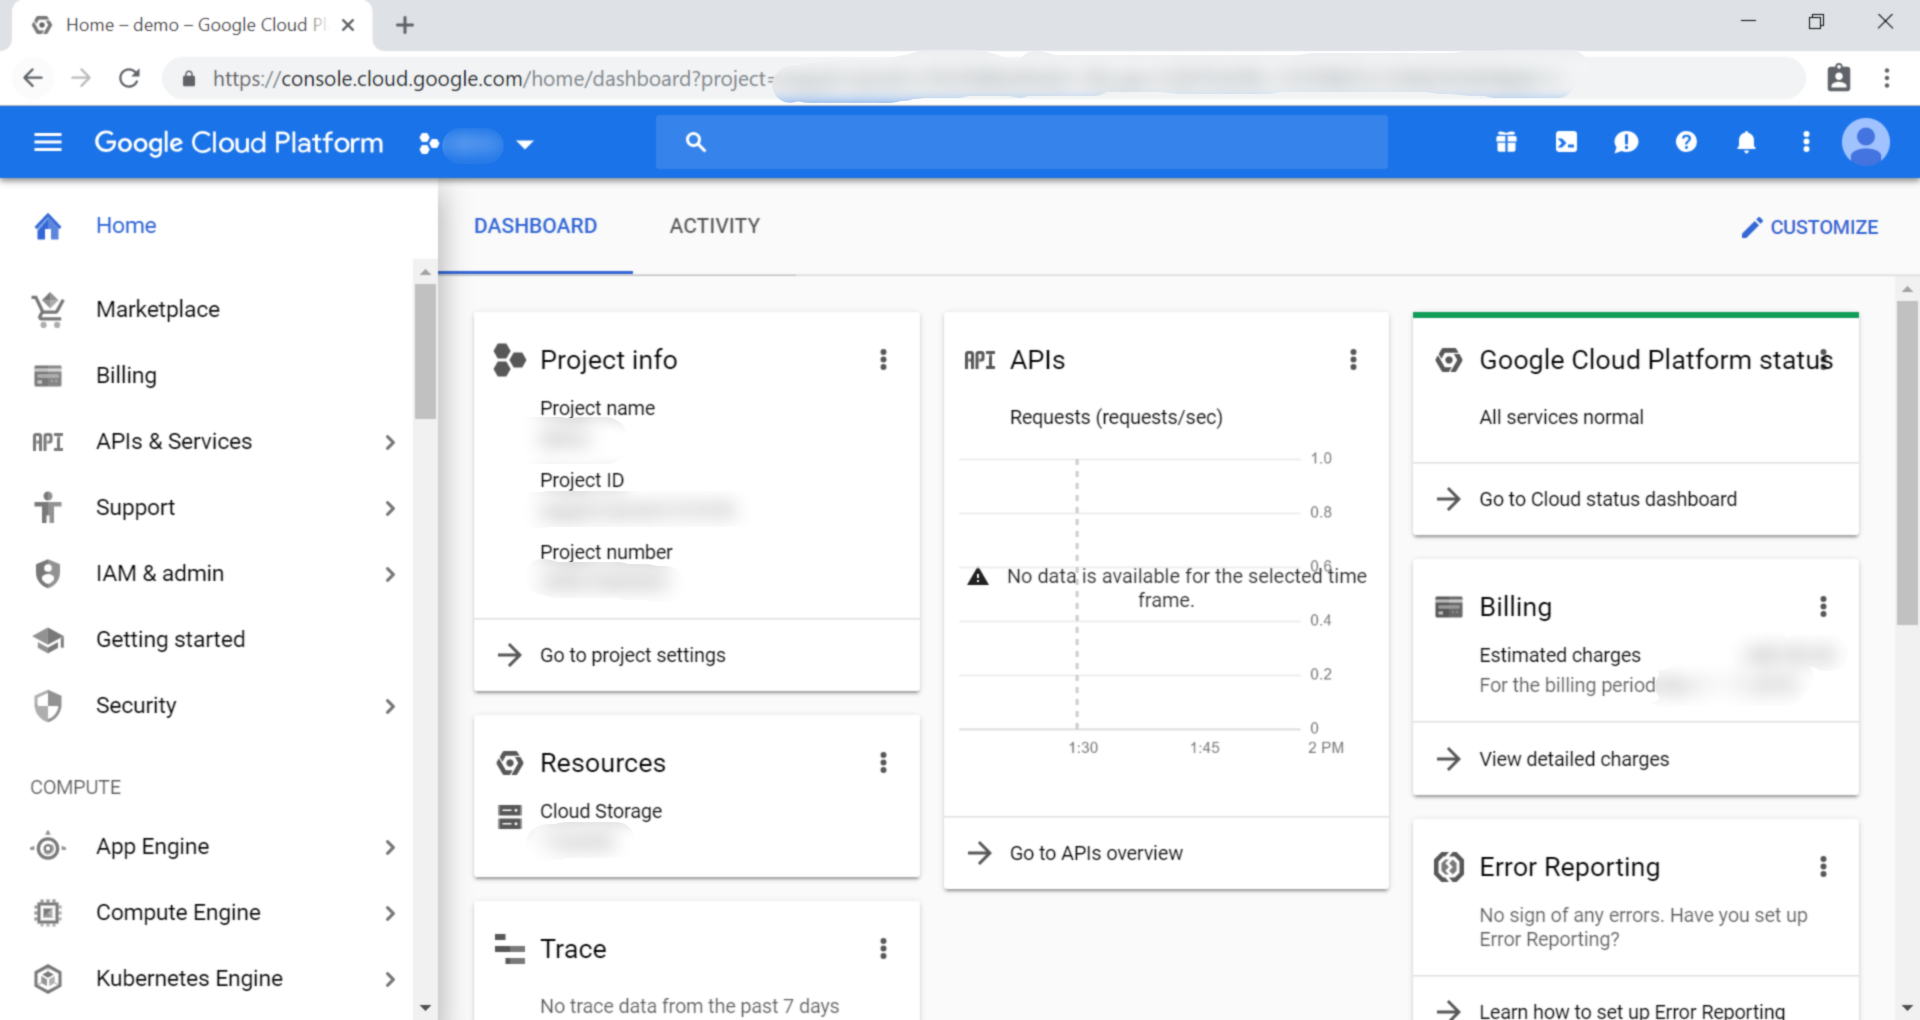
\includegraphics[width=0.6\columnwidth]{images/appendixA/GCP-console.PNG}
	      		\footcaption{Google Cloud Platform console}
	      	\end{figure}
	      \end{center}
	      \footnotetext{Source: \url{https://cloud.google.com/}} 
	\item Create \textit{Google Cloud Storage Bucket}. From the console, open navigation menu, and select \textit{Storage}
	      \begin{center}
	      	\begin{figure}[H]
	      		\centering
	      		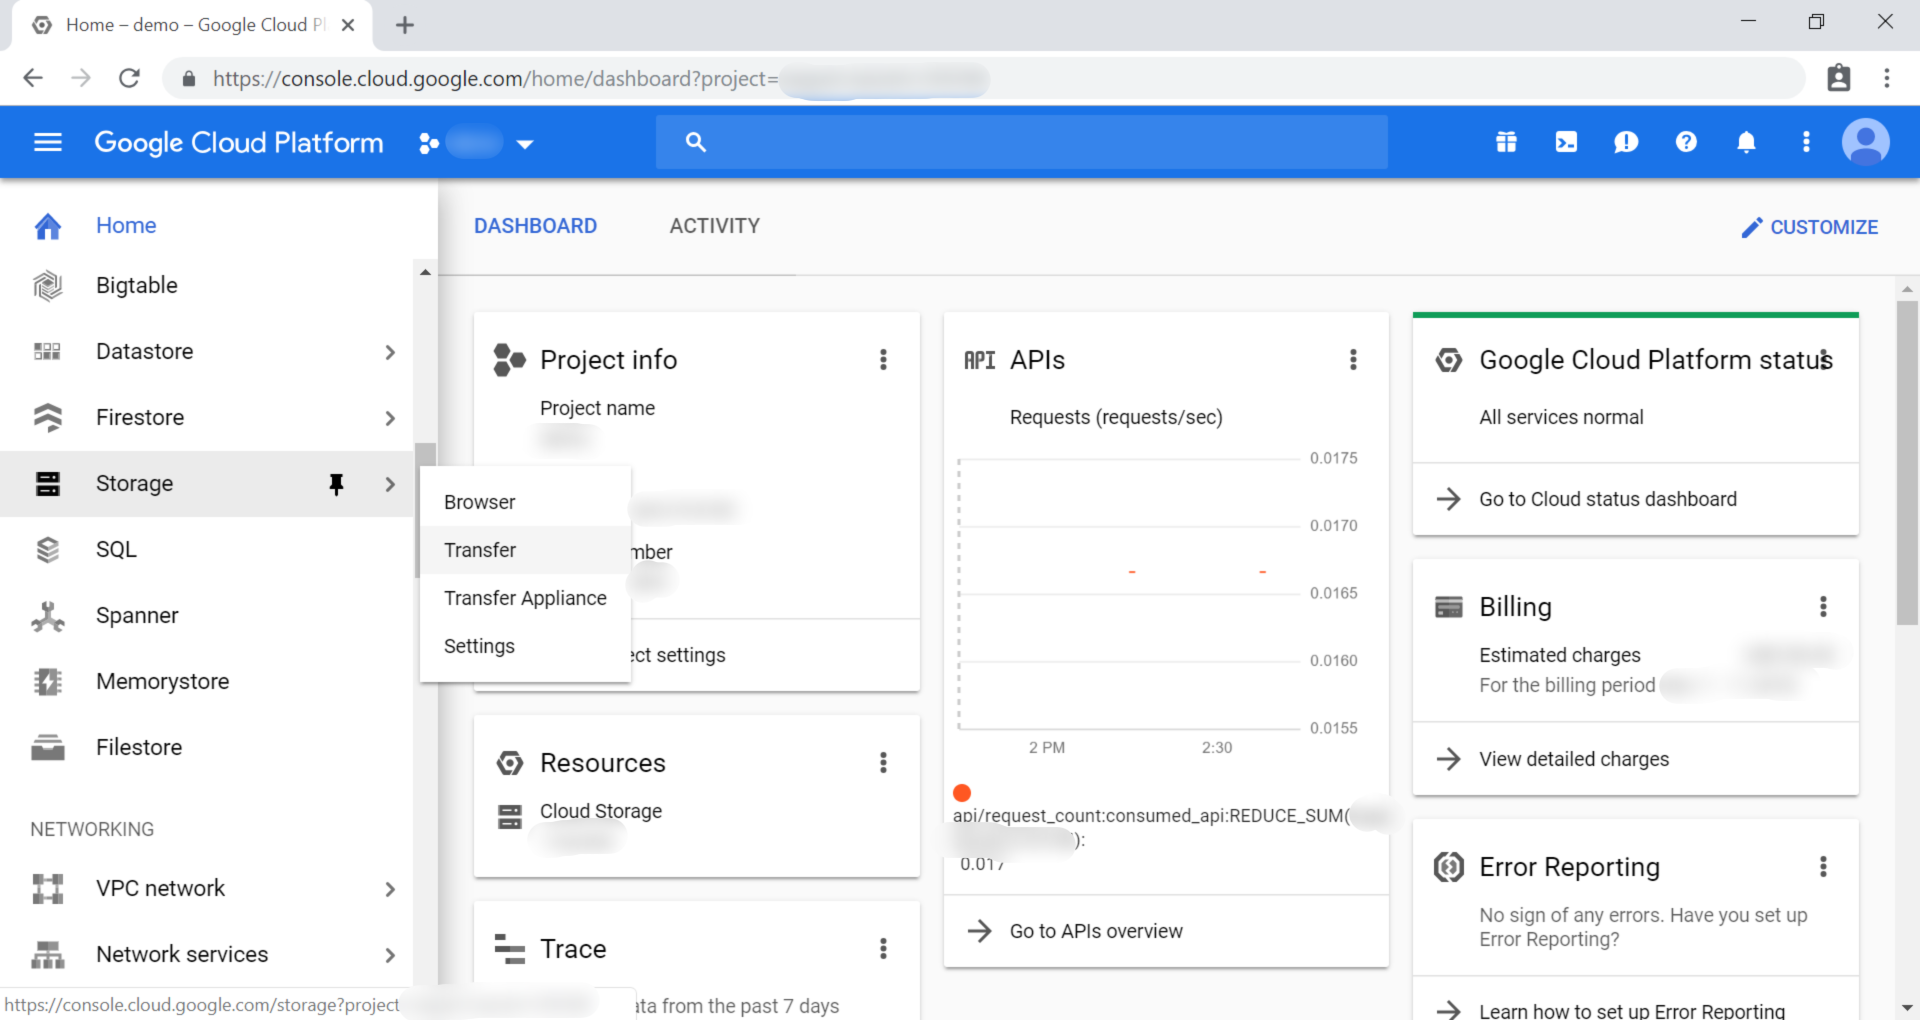
\includegraphics[width=0.6\columnwidth]{images/appendixA/GCP-navigate-Storage.PNG}
	      		\footcaption{Google Cloud Platform: Navigation Menu > Storage}
	      	\end{figure}
	      \end{center}
	      \footnotetext{Source: \url{https://cloud.google.com/}} 
	\item Click \textit{Create bucket} button and provide required information
	      \begin{center}
	      	\begin{figure}[H]
	      		\centering
	      		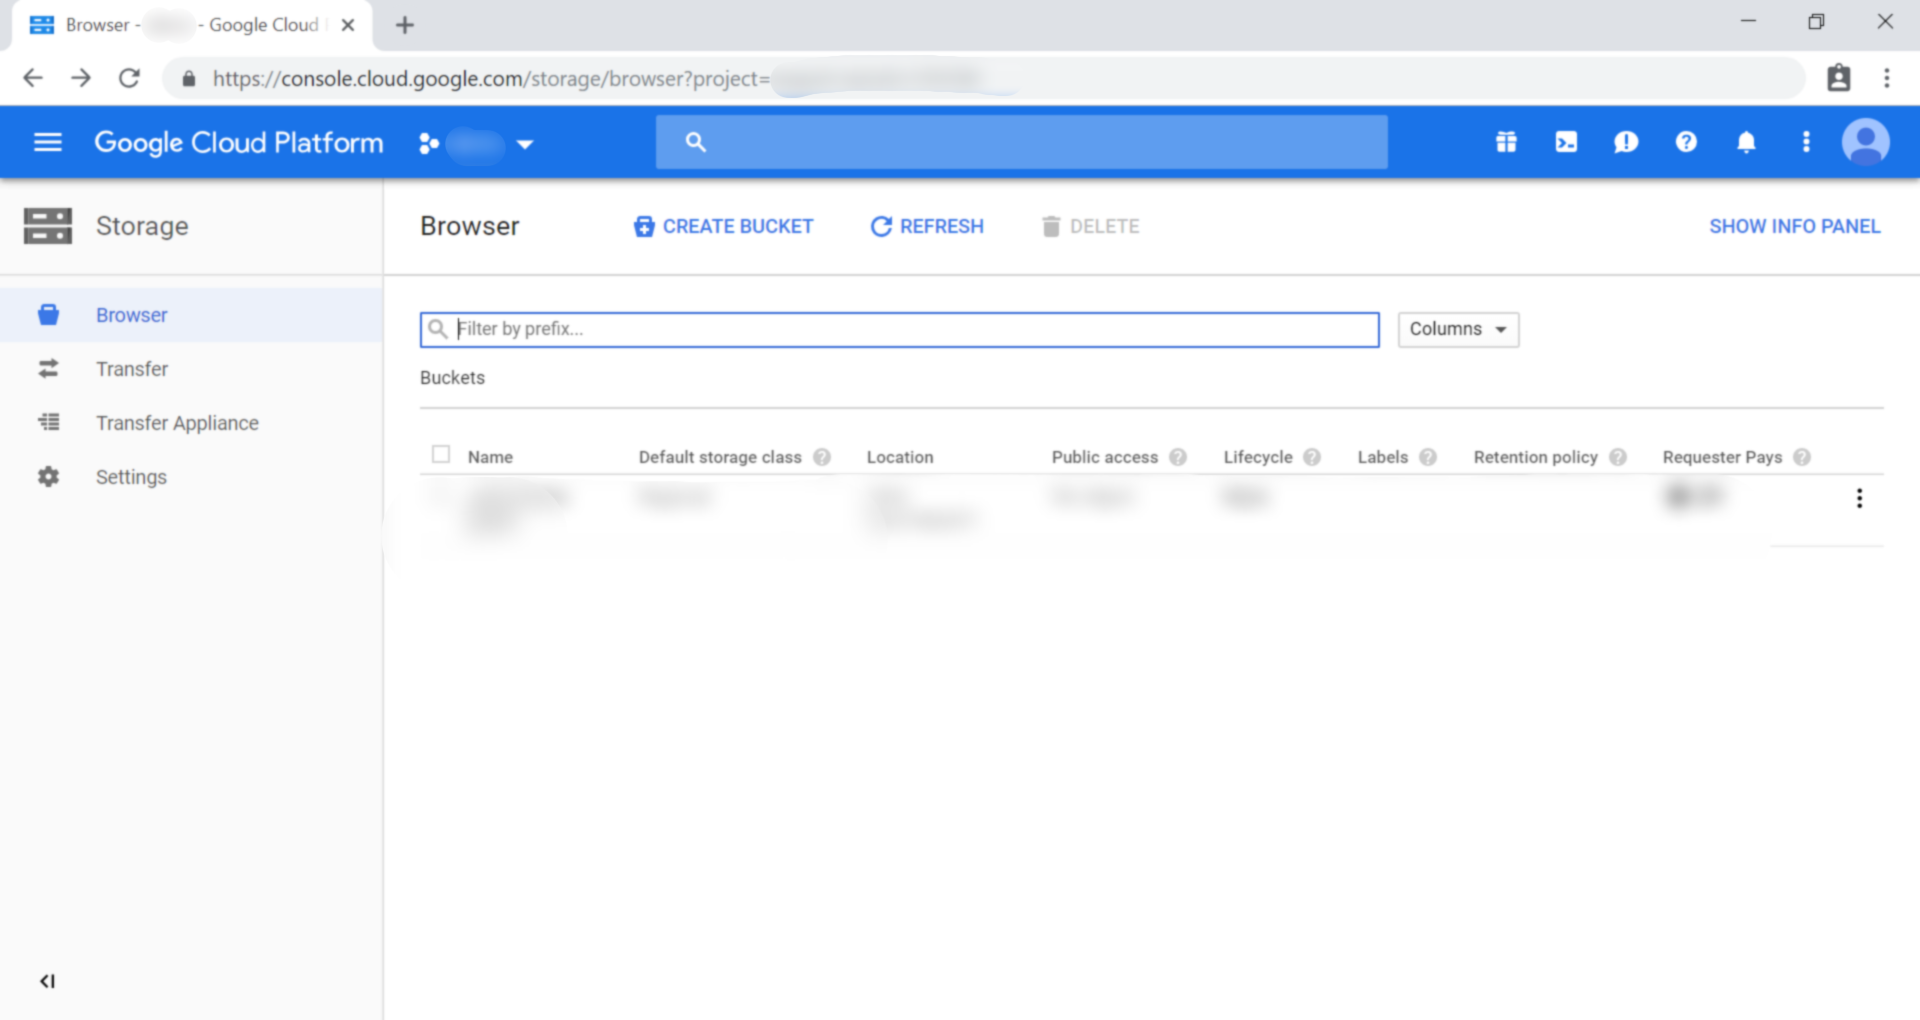
\includegraphics[width=0.6\columnwidth]{images/appendixA/GCP-Storage.PNG}
	      		\footcaption{Google Cloud Storage Management}
	      	\end{figure}
	      	\begin{figure}[H]
	      		\centering
	      		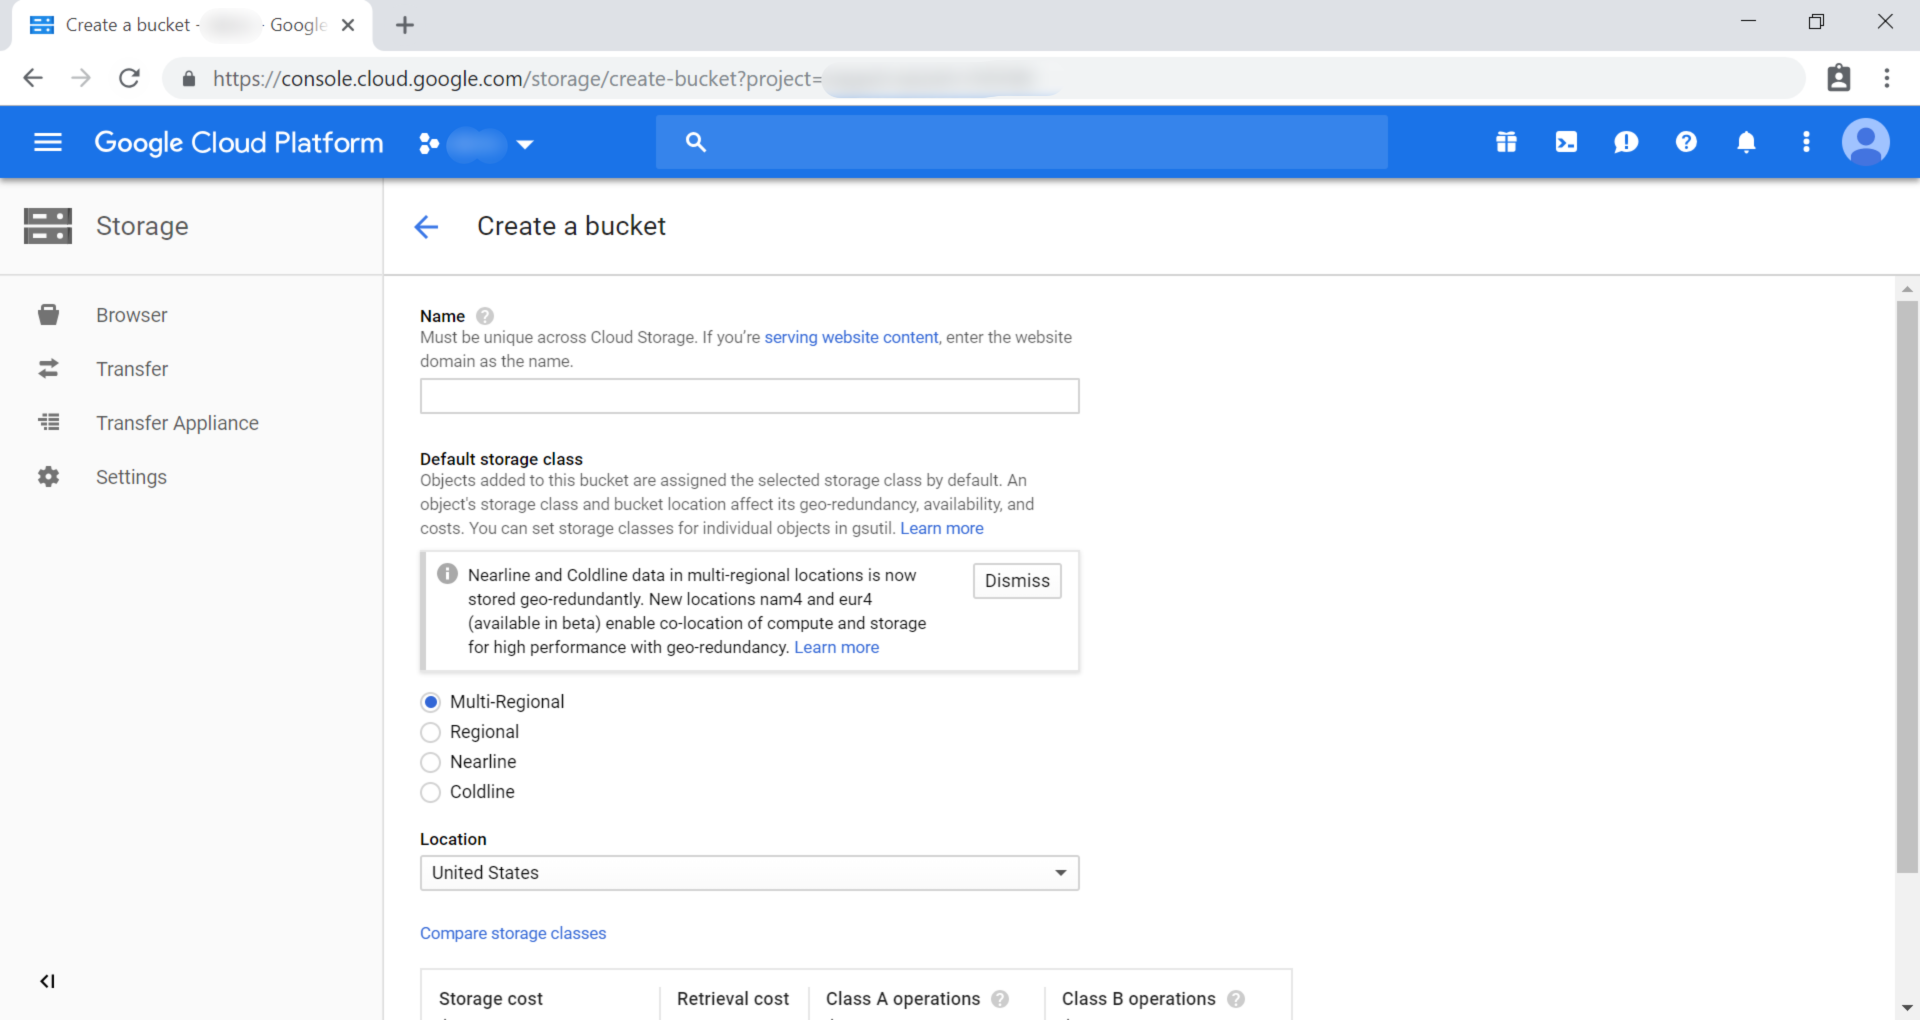
\includegraphics[width=0.6\columnwidth]{images/appendixA/GCP-Storage-create-bucket.PNG}
	      		\footcaption{Google Cloud Storage: Create Bucket}
	      	\end{figure}
	      \end{center}
	      \footnotetext{Source: \url{https://cloud.google.com/}}
	\item Following instruction in \href{https://cloud.google.com/iam/docs/creating-managing-service-accounts#creating_a_service_account}{this page} to create a \textit{Service Account} 
	\item Following instruction in \href{https://cloud.google.com/iam/docs/granting-roles-to-service-accounts#granting_access_to_a_service_account_for_a_resource}{this page} to grant role \textit{Storage Admin} for created \textit{Service Account}
	\item Following instruction in \href{https://cloud.google.com/iam/docs/creating-managing-service-account-keys#creating_service_account_keys}{this page} to create a \textit{Service Account key}. Download and keep 
\end{enumerate}

\section{Source code}
\chapter{User manual}
\section{Verifying account}
1. Login with your account or register new account. 
\begin{center}
    \begin{figure}[H]
    \centering
    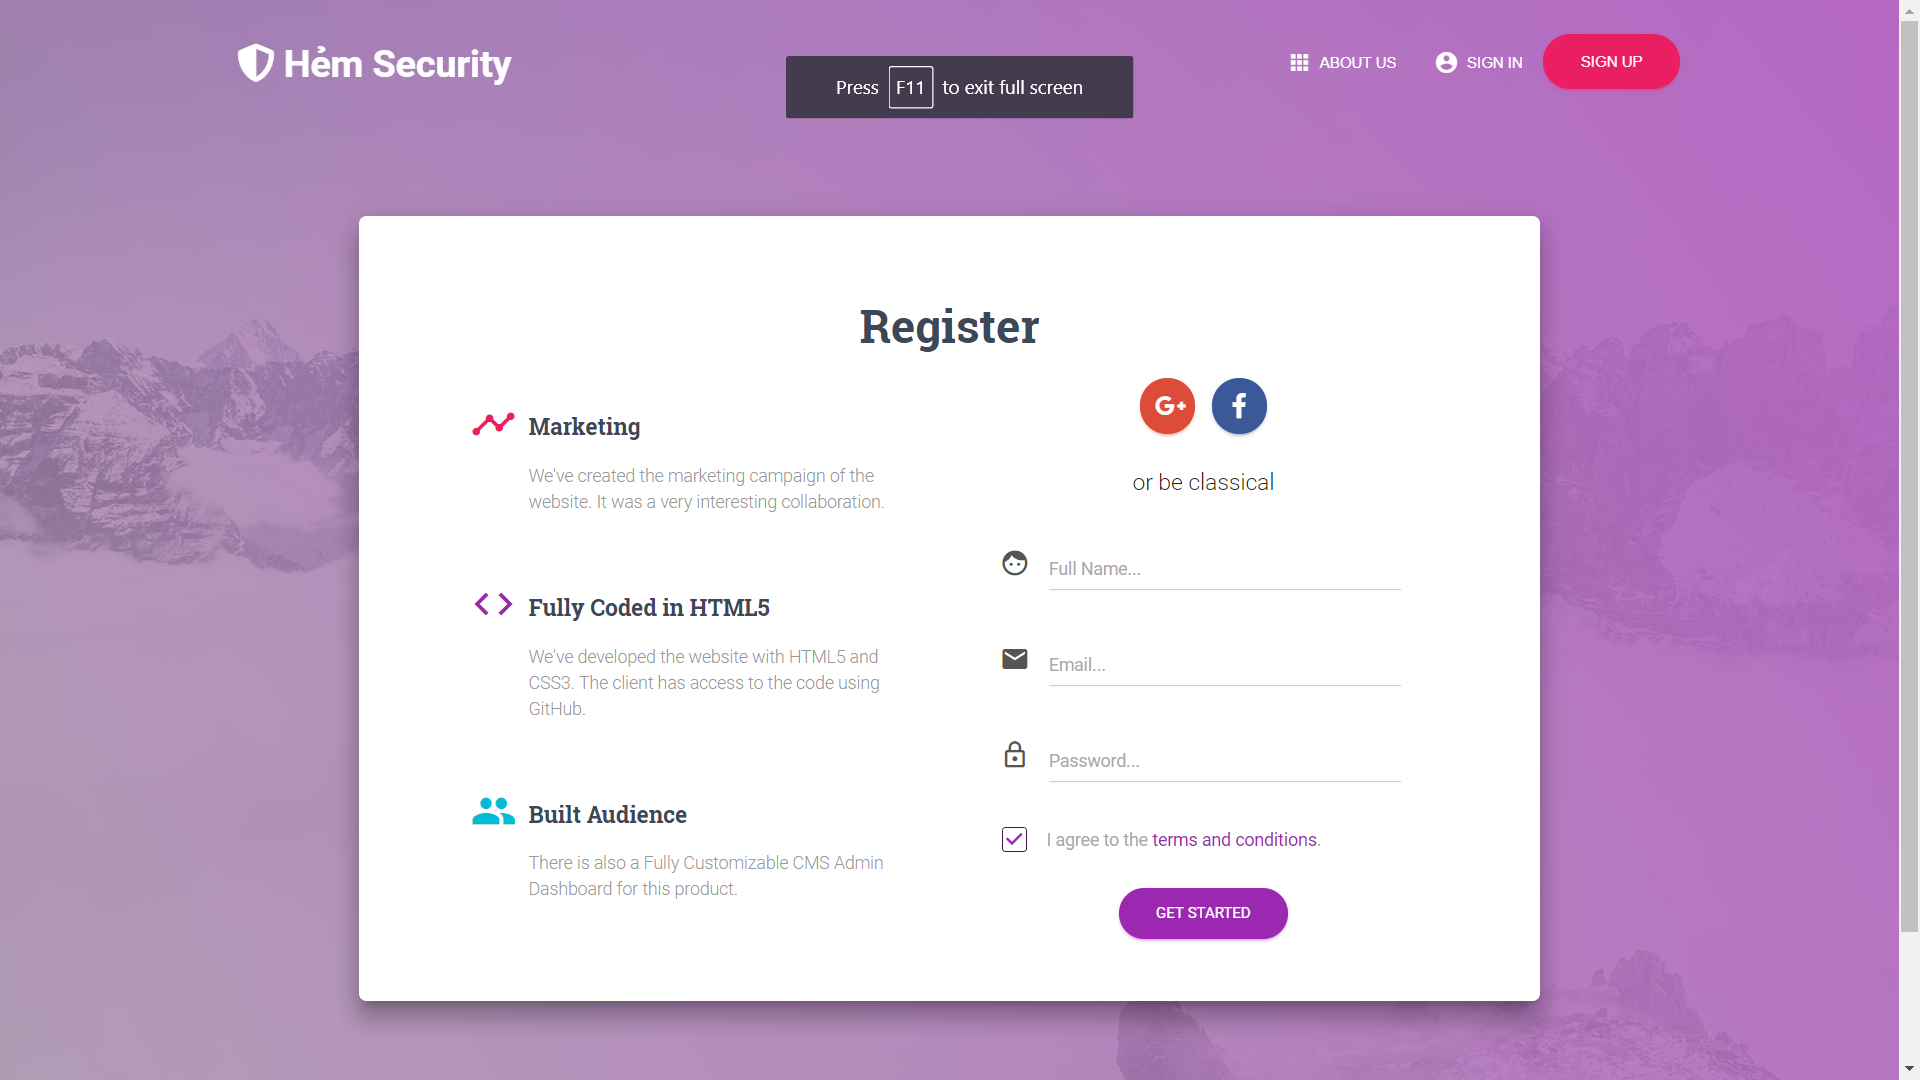
\includegraphics[width=1\columnwidth]{images/chap6/instruction1.png}
    \footcaption{Homepage}
    \label{}
    \end{figure}
\end{center}
2. Unverified account is unable to use most of the features, verify your account by clicking your name to go to your profile page
\begin{center}
    \begin{figure}[H]
    \centering
    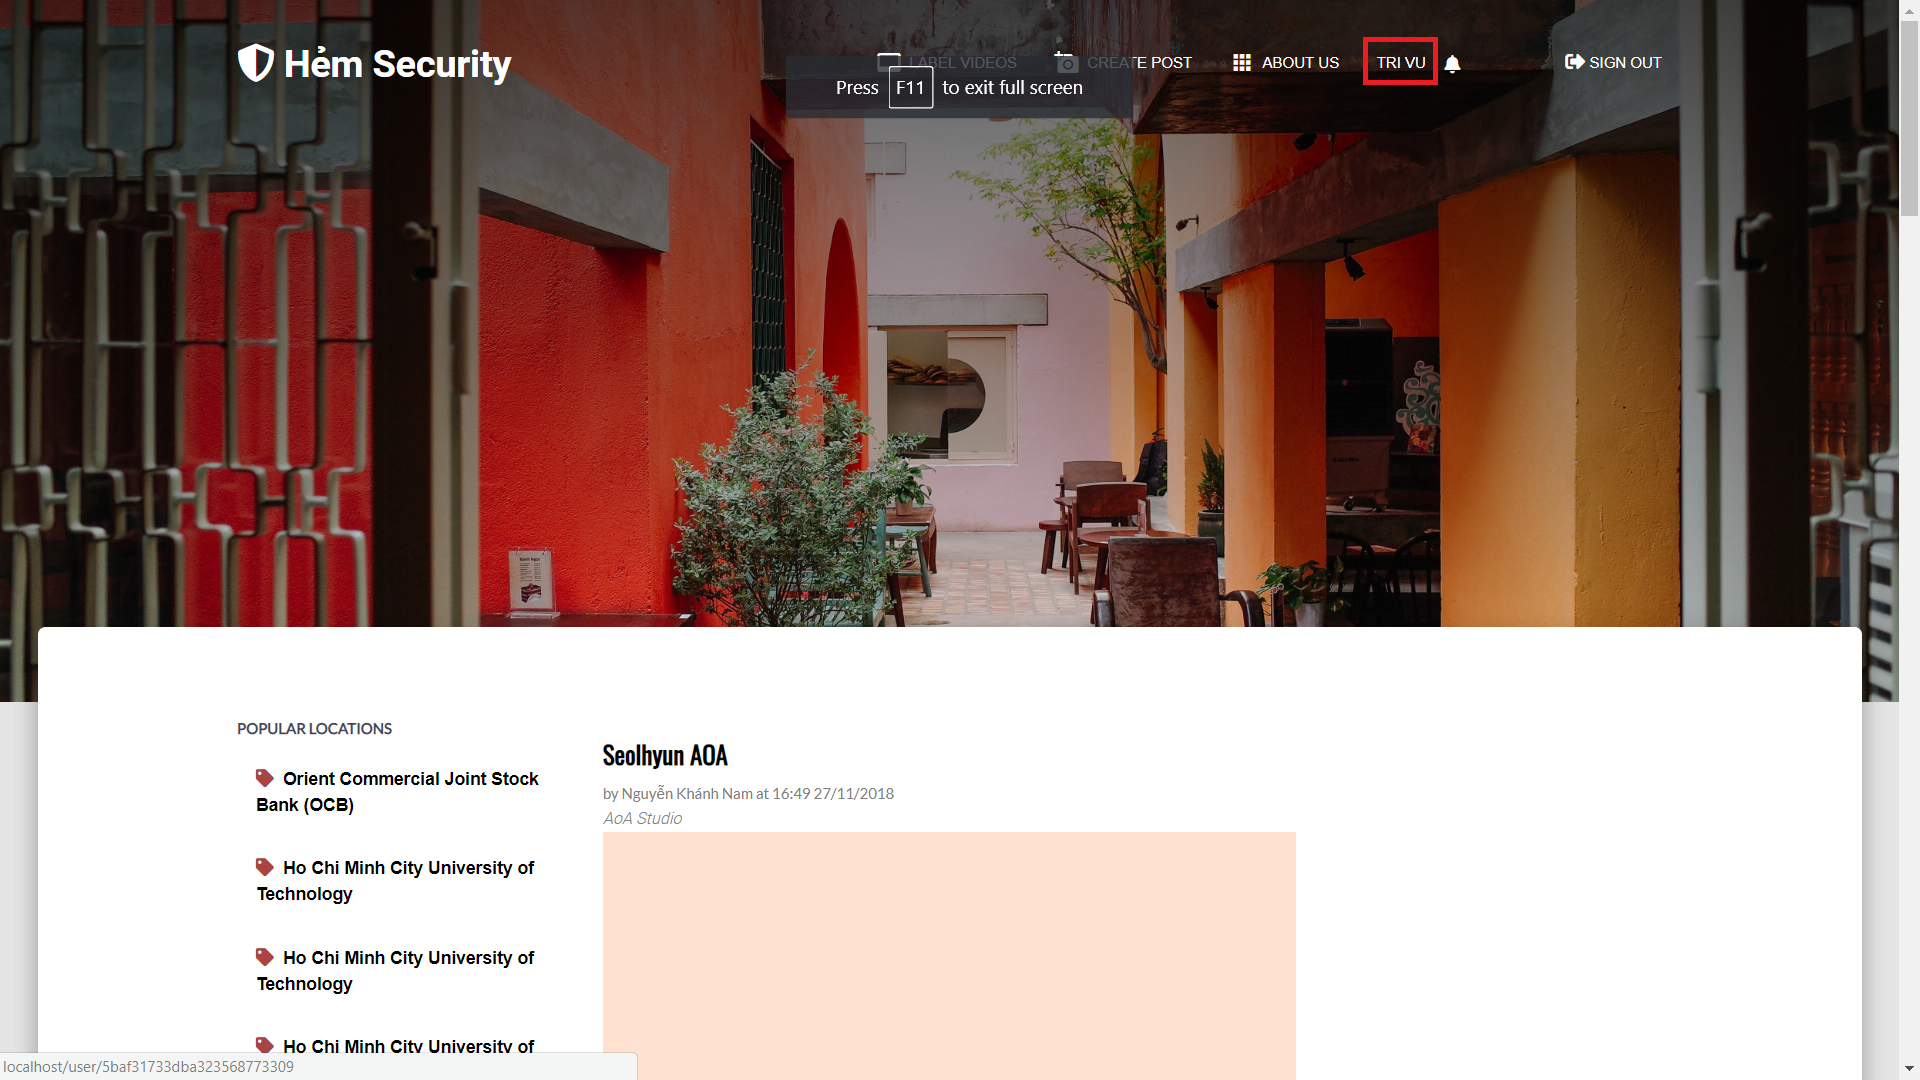
\includegraphics[width=1\columnwidth]{images/chap6/instruction2.png}
    \end{figure}
\end{center}
3. Enter your phone number to verify
\begin{center}
    \begin{figure}[H]
    \centering
    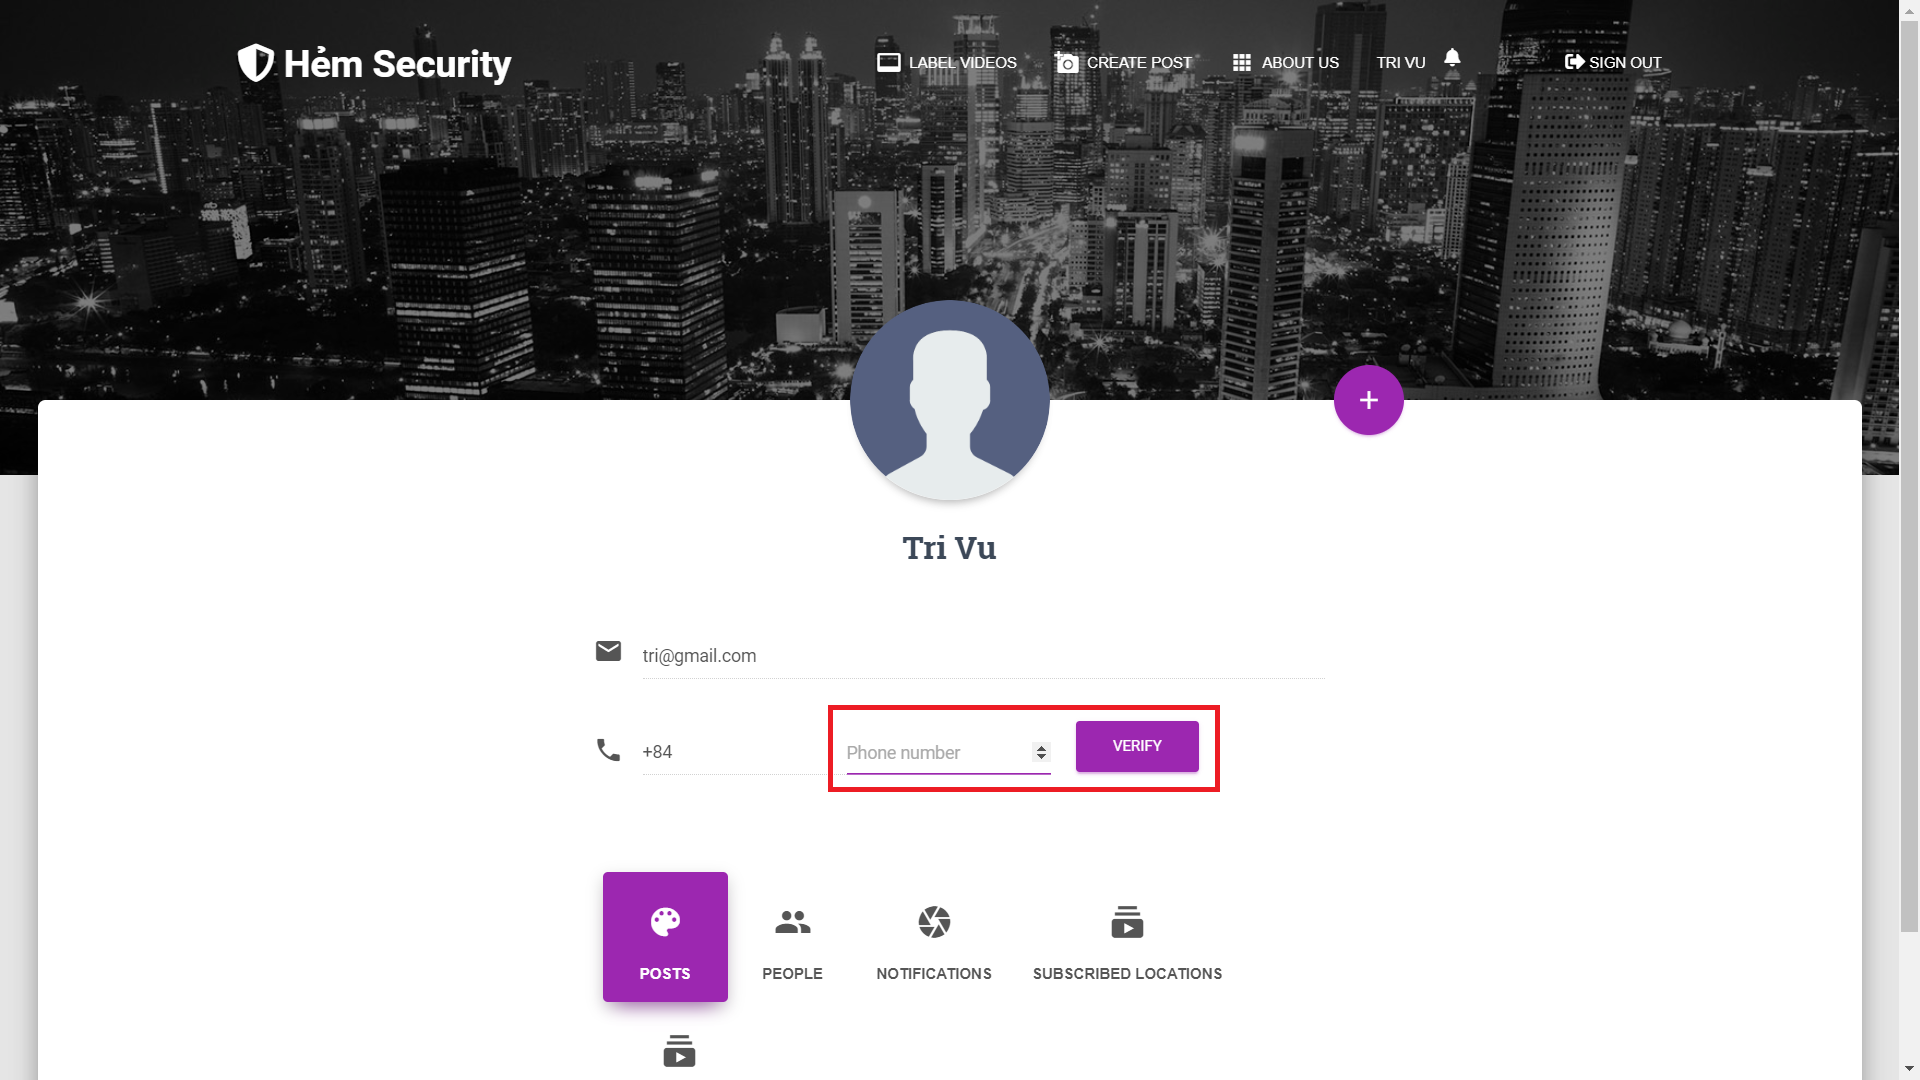
\includegraphics[width=1\columnwidth]{images/chap6/instruction3.png}
    \end{figure}
\end{center}
4. User can choose either to receive confirmation code by WhatsApp or SMS. Enter your code to finish verifying.
\begin{center}
    \begin{figure}[H]
    \centering
    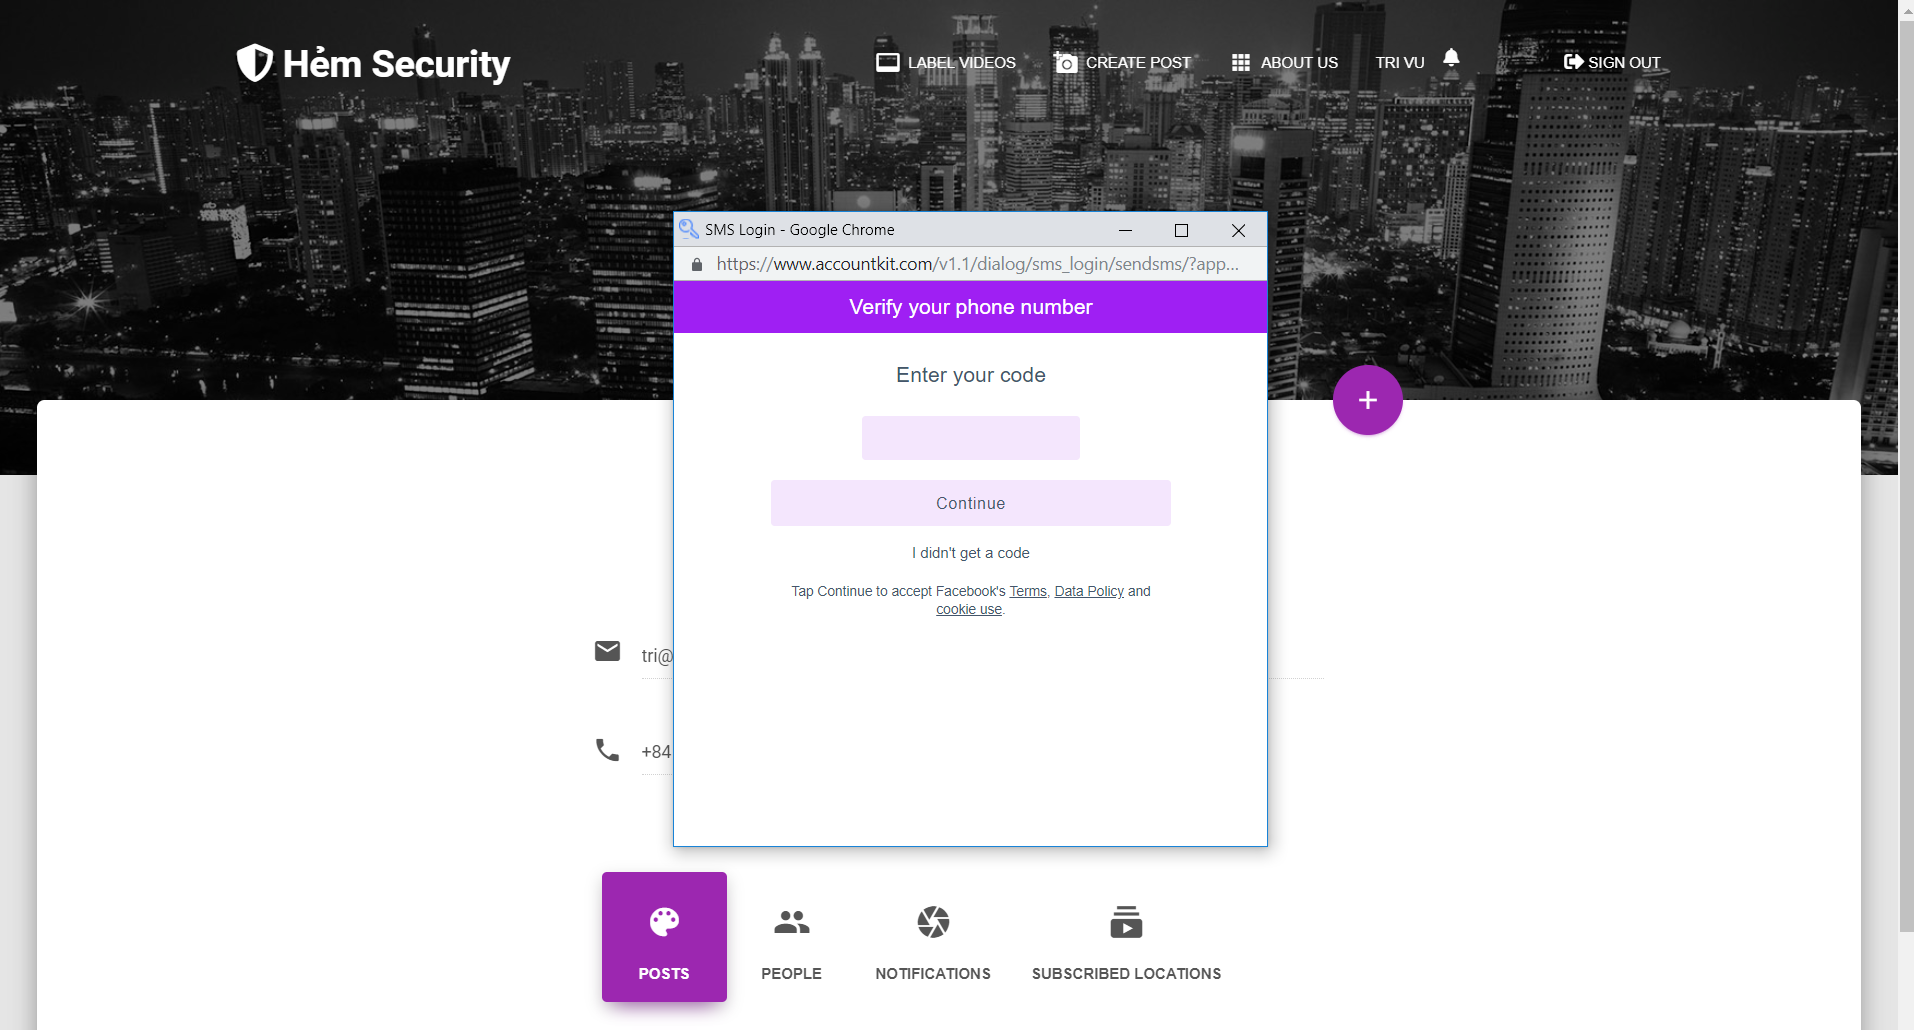
\includegraphics[width=1\columnwidth]{images/chap6/instruction4.png}
    \end{figure}
\end{center}
\section{Label video}
1. Go to "Label video" page
\begin{center}
    \begin{figure}[H]
    \centering
    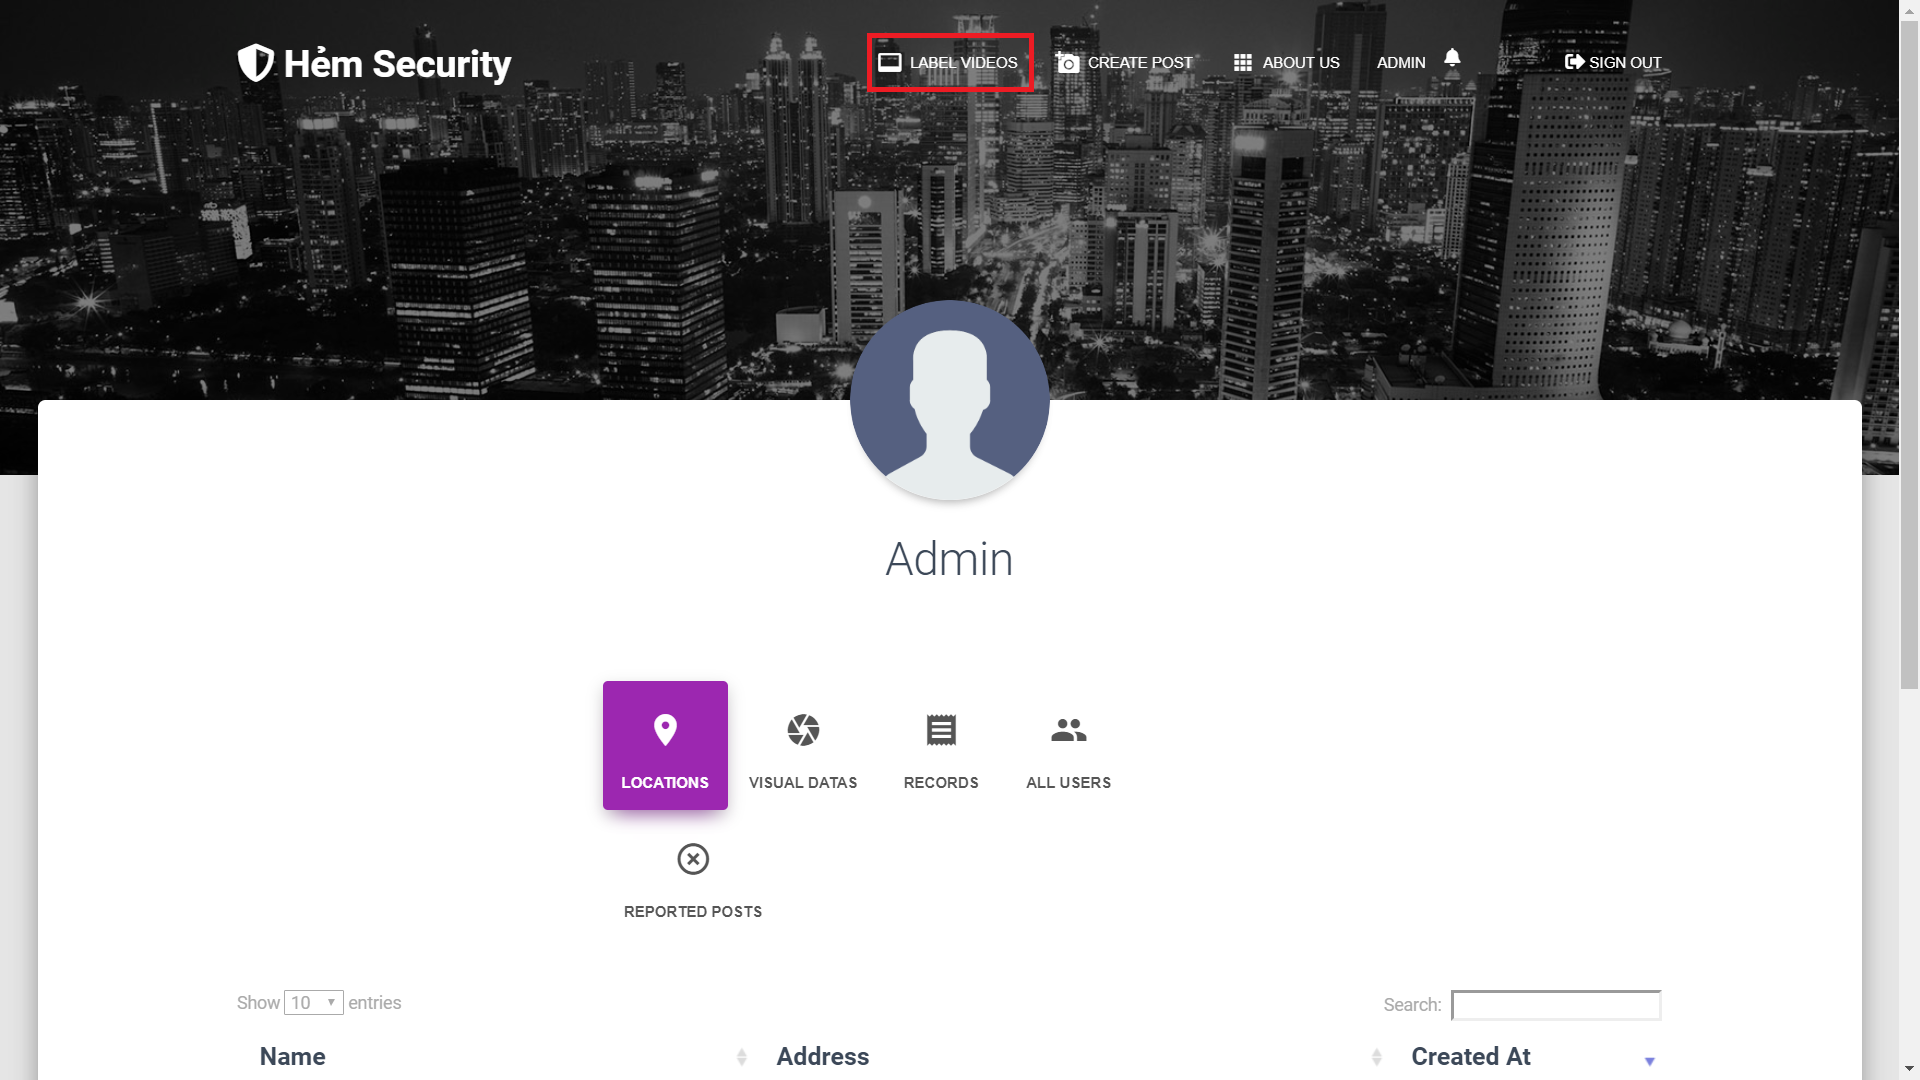
\includegraphics[width=1\columnwidth]{images/chap6/instruction5.png}
    \end{figure}
\end{center}
2. Choose either "Suspicious" or "Not suspicious". 
\begin{center}
    \begin{figure}[H]
    \centering
    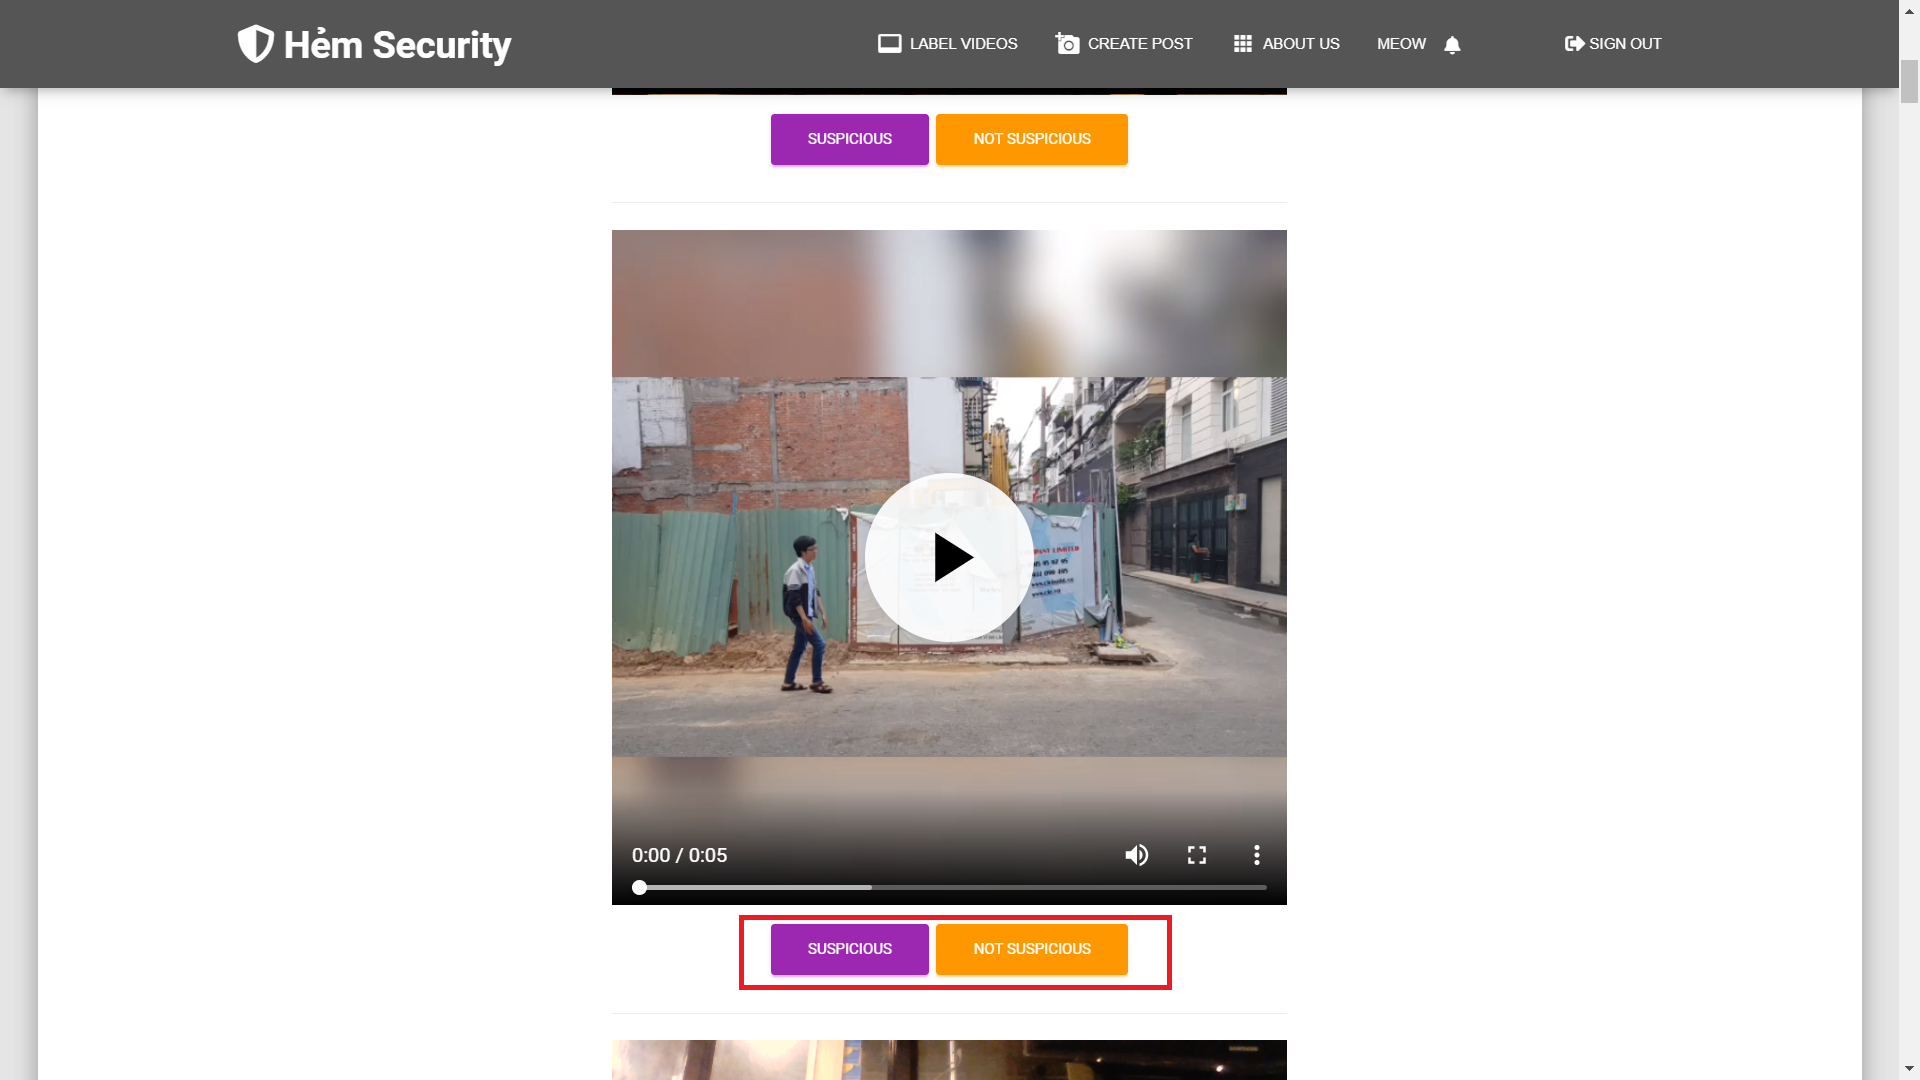
\includegraphics[width=1\columnwidth]{images/chap6/instruction6.png}
    \end{figure}
\end{center}
\section{Create post}
1. Go to "Create post" page
\begin{center}
    \begin{figure}[H]
    \centering
    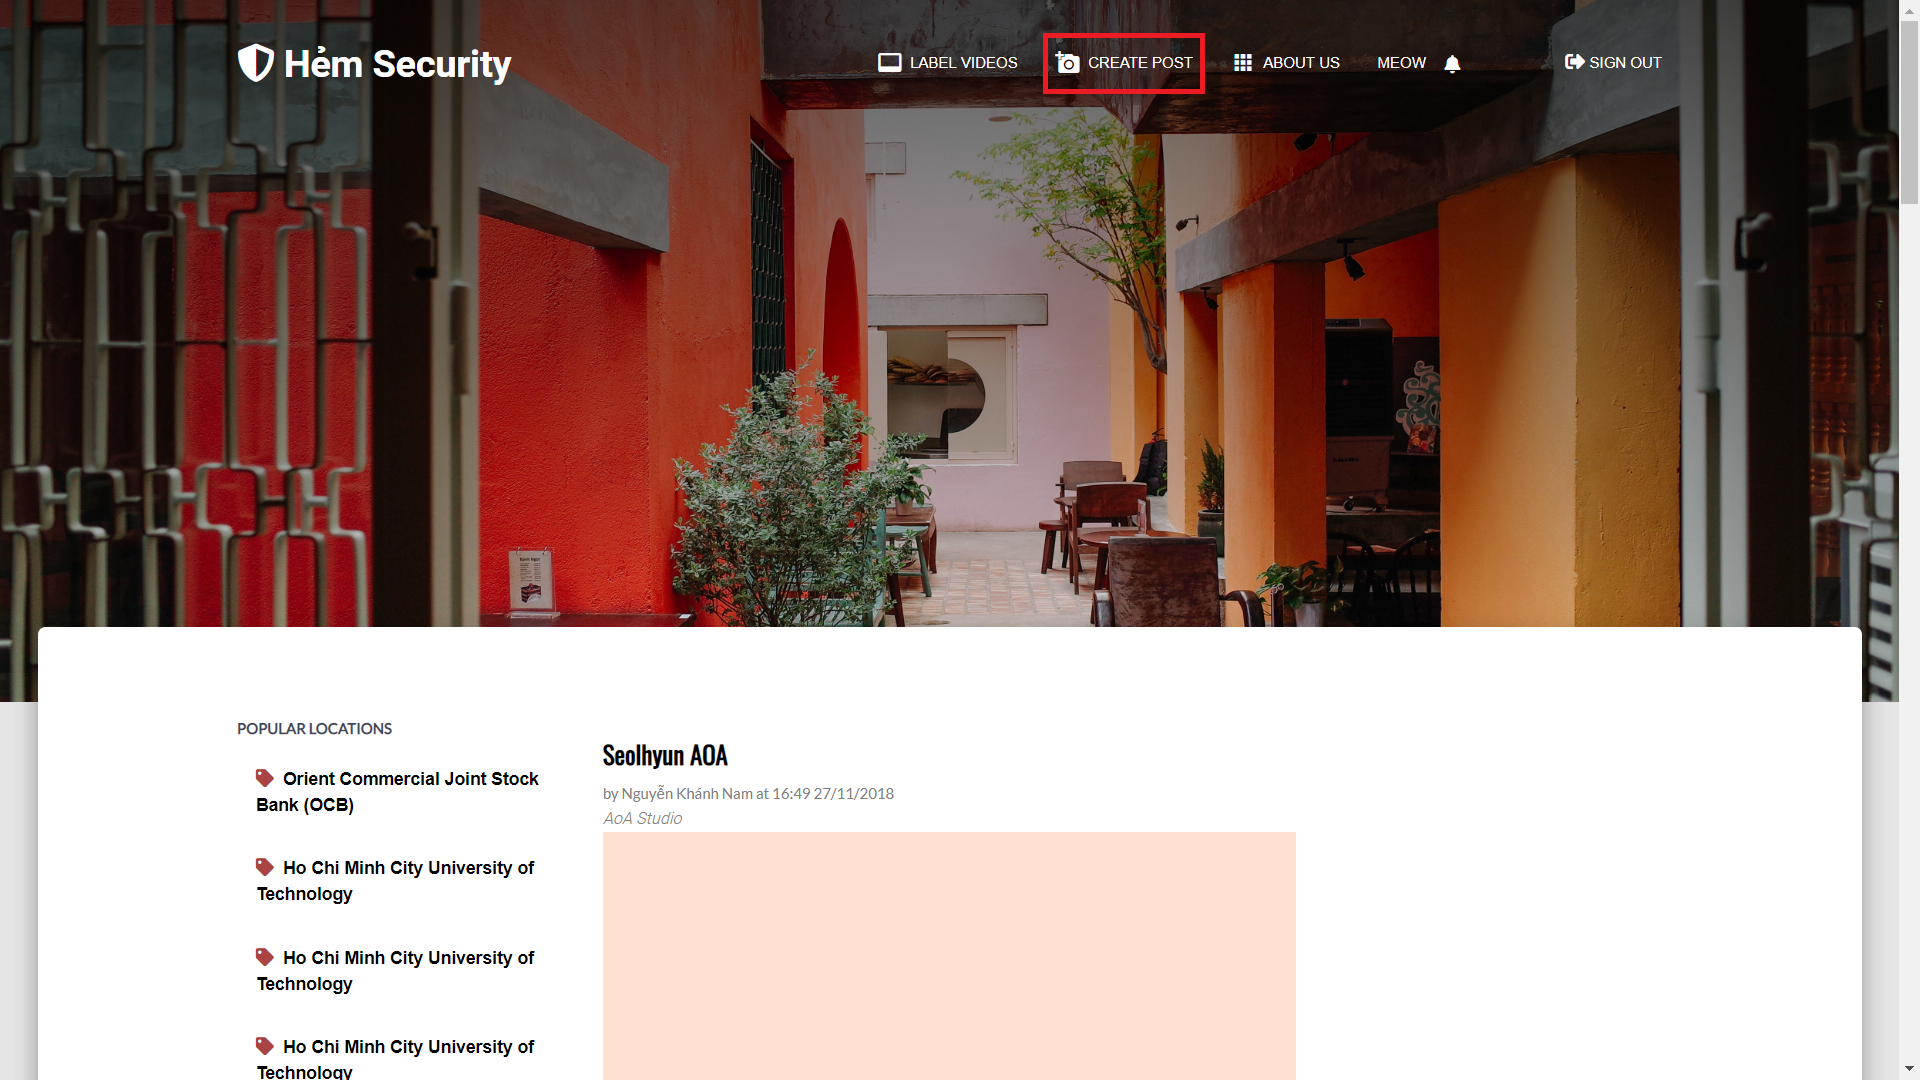
\includegraphics[width=1\columnwidth]{images/chap6/instruction7.png}
    \end{figure}
\end{center}
2. Fill in the form to and click "Create". 
\begin{center}
    \begin{figure}[H]
    \centering
    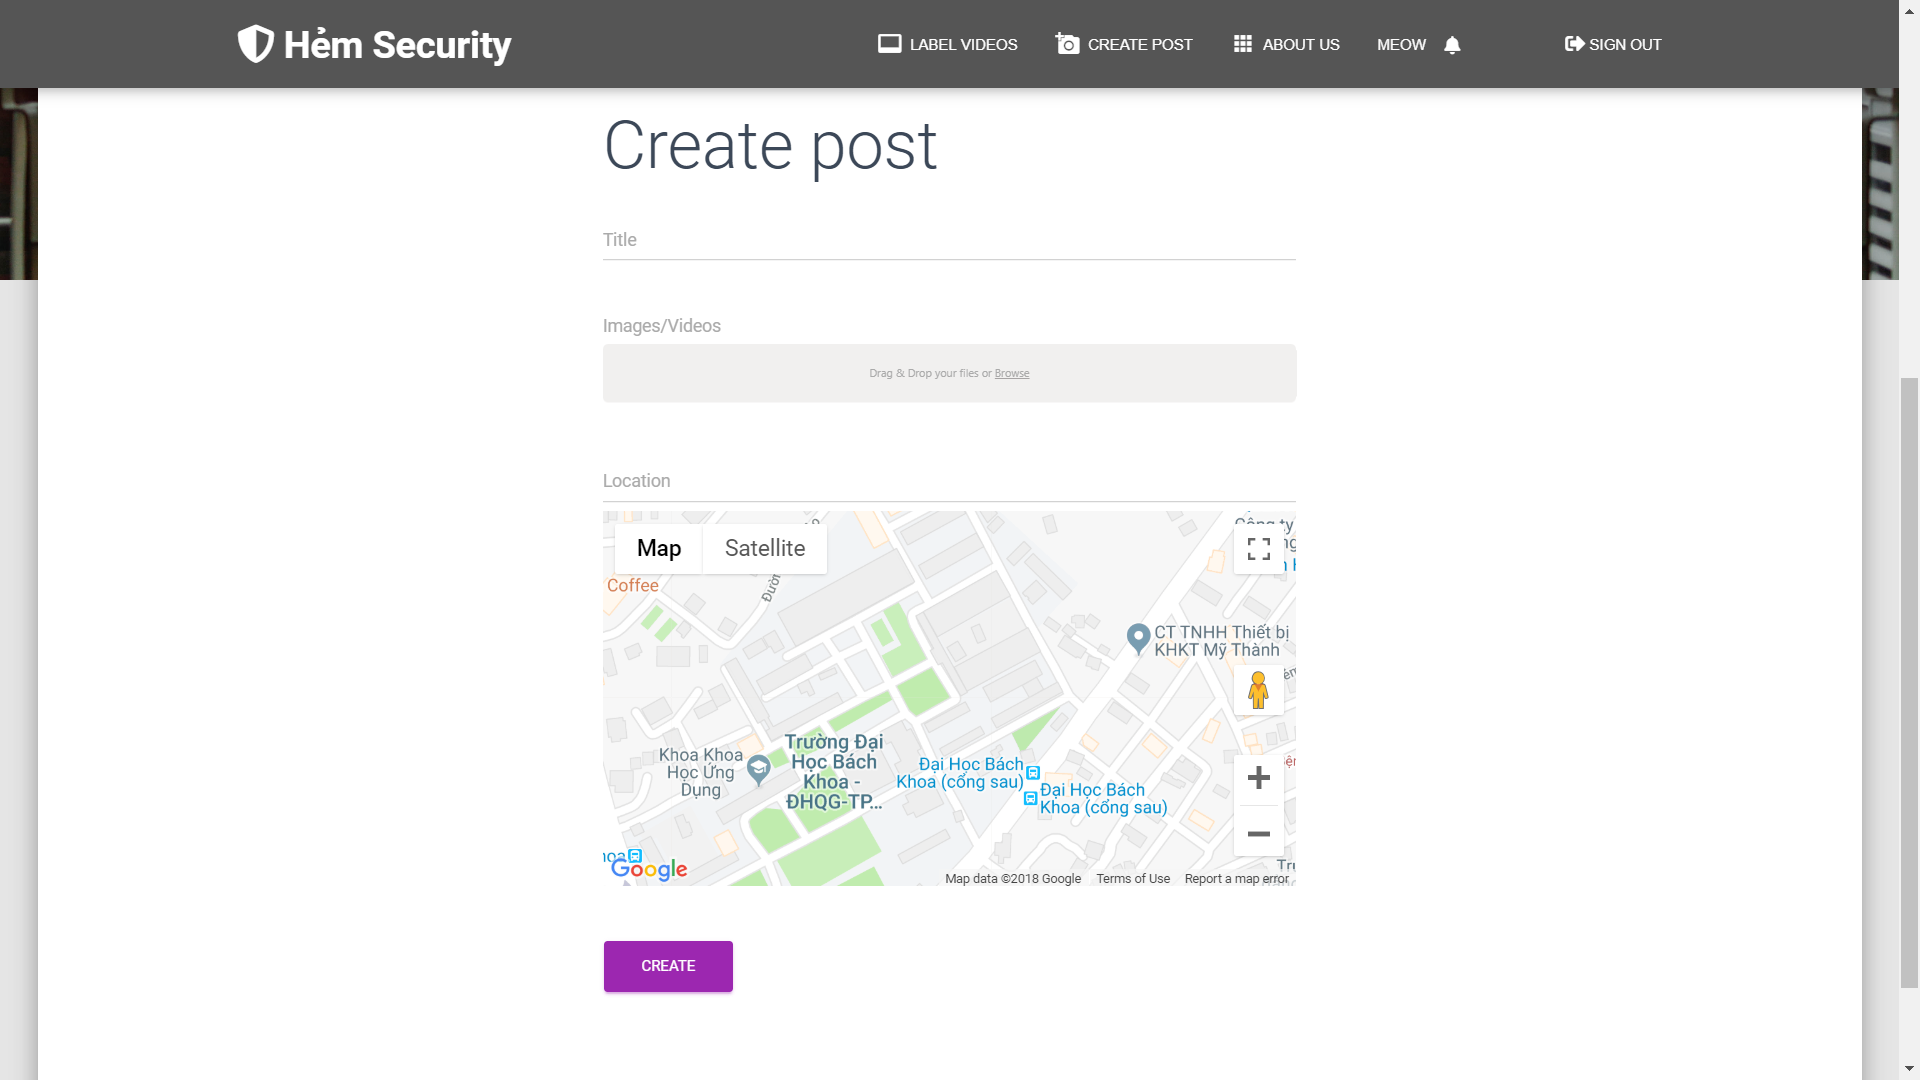
\includegraphics[width=1\columnwidth]{images/chap6/instruction8.png}
    \footcaption{Create post form}
    \end{figure}
\end{center}
\section{Subscribe a location}
1. Go to profile page and choose "All locations" tab
\begin{center}
    \begin{figure}[H]
    \centering
    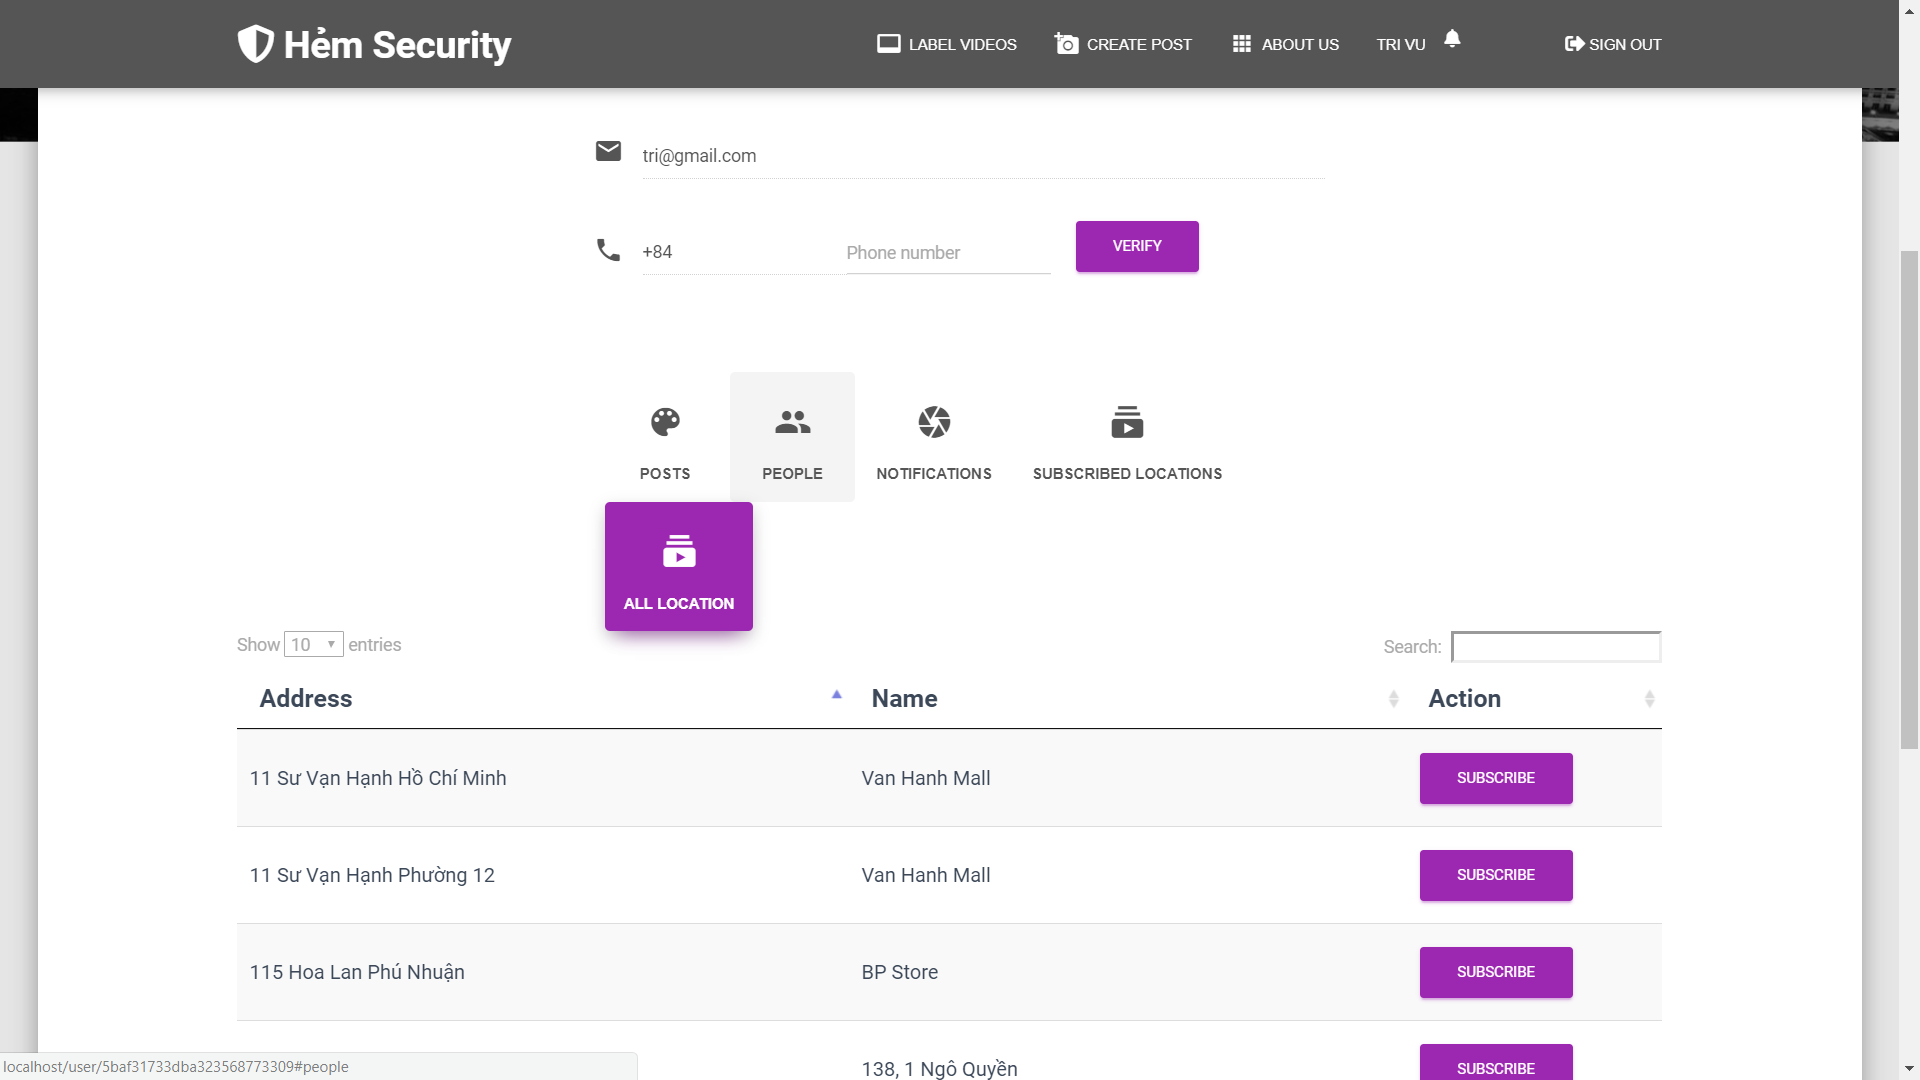
\includegraphics[width=1\columnwidth]{images/chap6/instruction9.png}
    \end{figure}
\end{center}
2. Choose a location to subscribe from the list. User will receive notification about suspicious behavior around subscribed location within a radius of 1 kilometer.   
\begin{center}
    \begin{figure}[H]
    \centering
    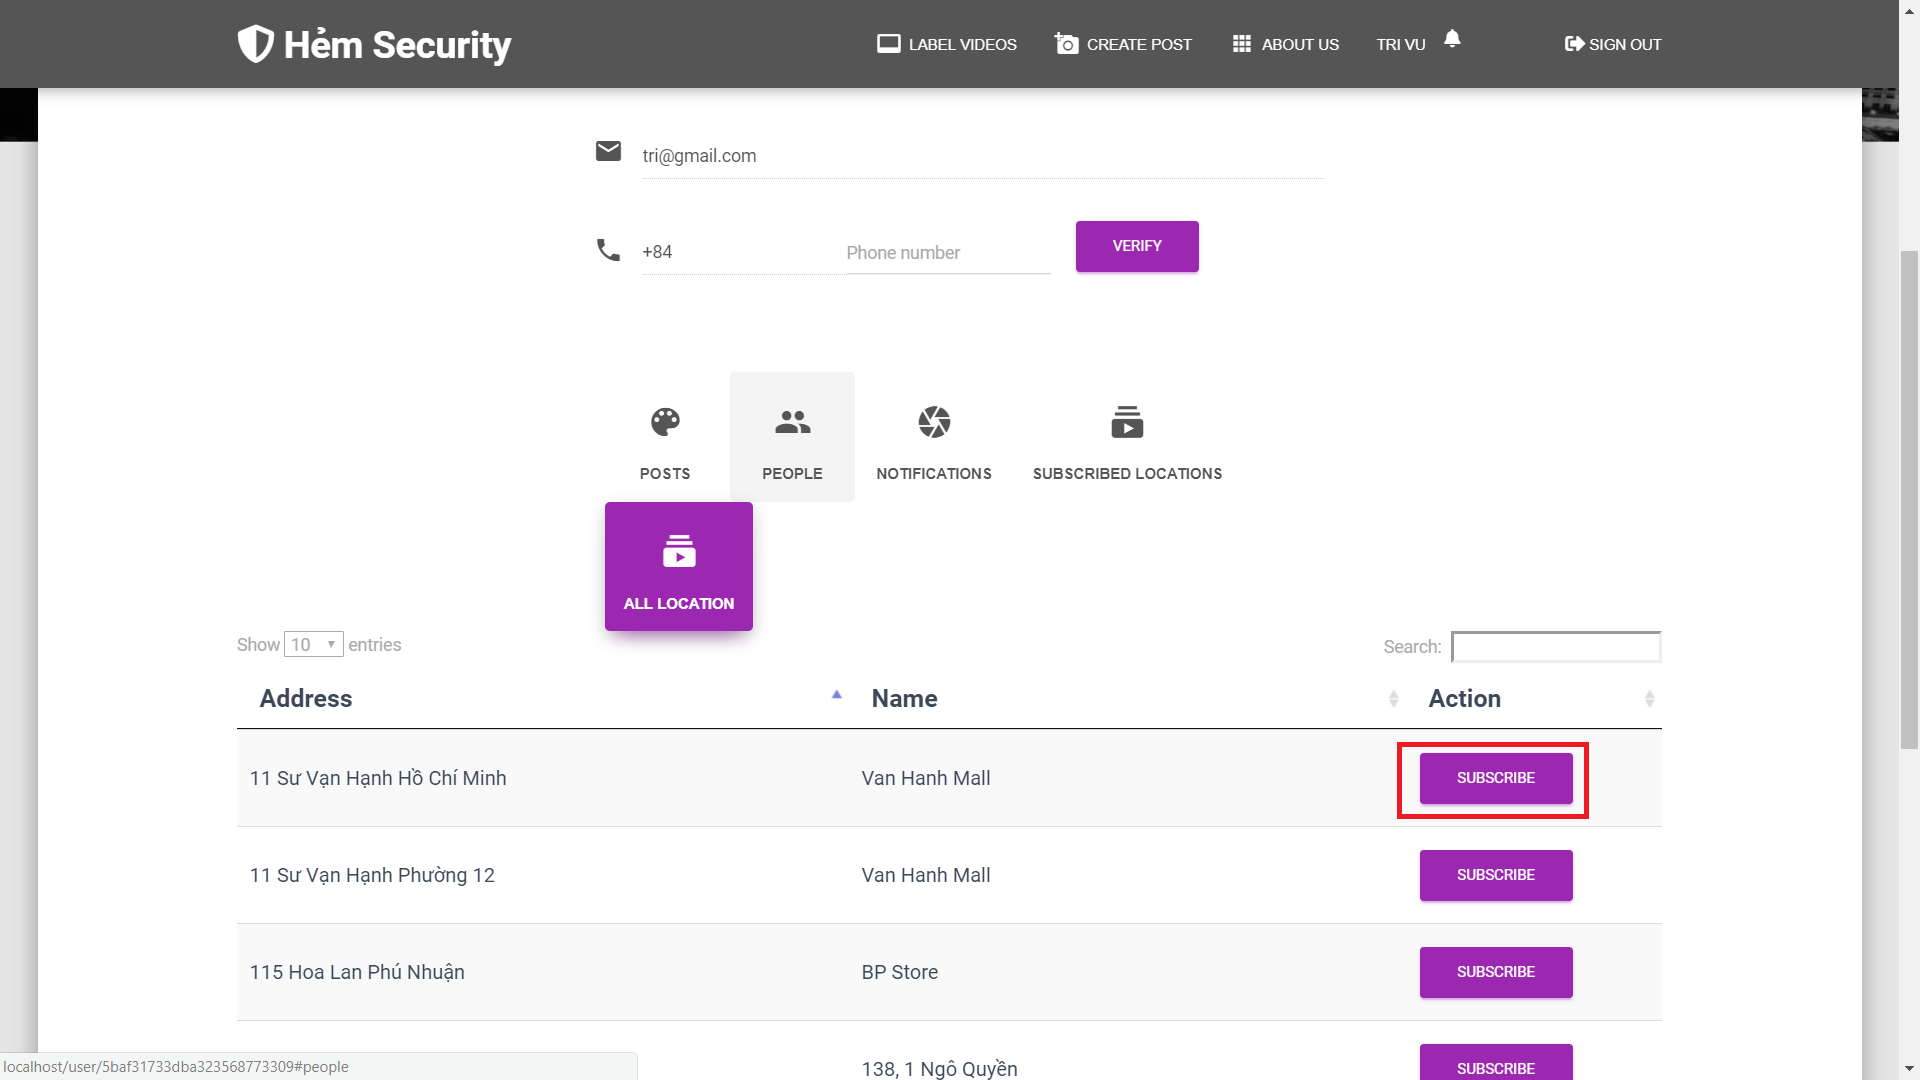
\includegraphics[width=1\columnwidth]{images/chap6/instruction10.png}
    \end{figure}
\end{center}

